%
% File: thesis.tex
% Created: 月 11 30 08:00 午後 2015 東京 (標準時)
% Last Change: 月 11 30 08:00 午後 2015 東京 (標準時)
%
%%% jdummy.def
%
\DeclareRelationFont{JY1}{mc}{it}{}{OT1}{cmr}{it}{}
\DeclareRelationFont{JT1}{mc}{it}{}{OT1}{cmr}{it}{}
\DeclareFontShape{JY1}{mc}{m}{it}{<5> <6> <7> <8> <9> <10> sgen*min
    <10.95><12><14.4><17.28><20.74><24.88> min10
    <-> min10}{}
\DeclareFontShape{JT1}{mc}{m}{it}{<5> <6> <7> <8> <9> <10> sgen*tmin
    <10.95><12><14.4><17.28><20.74><24.88> tmin10
    <-> tmin10}{}
\DeclareRelationFont{JY1}{mc}{sl}{}{OT1}{cmr}{sl}{}
\DeclareRelationFont{JT1}{mc}{sl}{}{OT1}{cmr}{sl}{}
\DeclareFontShape{JY1}{mc}{m}{sl}{<5> <6> <7> <8> <9> <10> sgen*min
    <10.95><12><14.4><17.28><20.74><24.88> min10
    <-> min10}{}
\DeclareFontShape{JT1}{mc}{m}{sl}{<5> <6> <7> <8> <9> <10> sgen*tmin
    <10.95><12><14.4><17.28><20.74><24.88> tmin10
    <-> tmin10}{}
\DeclareRelationFont{JY1}{mc}{sc}{}{OT1}{cmr}{sc}{}
\DeclareRelationFont{JT1}{mc}{sc}{}{OT1}{cmr}{sc}{}
\DeclareFontShape{JY1}{mc}{m}{sc}{<5> <6> <7> <8> <9> <10> sgen*min
    <10.95><12><14.4><17.28><20.74><24.88> min10
    <-> min10}{}
\DeclareFontShape{JT1}{mc}{m}{sc}{<5> <6> <7> <8> <9> <10> sgen*tmin
    <10.95><12><14.4><17.28><20.74><24.88> tmin10
    <-> tmin10}{}
\DeclareRelationFont{JY1}{gt}{it}{}{OT1}{cmbx}{it}{}
\DeclareRelationFont{JT1}{gt}{it}{}{OT1}{cmbx}{it}{}
\DeclareFontShape{JY1}{mc}{bx}{it}{<5> <6> <7> <8> <9> <10> sgen*goth
    <10.95><12><14.4><17.28><20.74><24.88> goth10
    <-> goth10}{}
\DeclareFontShape{JT1}{mc}{bx}{it}{<5> <6> <7> <8> <9> <10> sgen*tgoth
    <10.95><12><14.4><17.28><20.74><24.88> tgoth10
    <-> tgoth10}{}
\DeclareRelationFont{JY1}{gt}{sl}{}{OT1}{cmbx}{sl}{}
\DeclareRelationFont{JT1}{gt}{sl}{}{OT1}{cmbx}{sl}{}
\DeclareFontShape{JY1}{mc}{bx}{sl}{<5> <6> <7> <8> <9> <10> sgen*goth
    <10.95><12><14.4><17.28><20.74><24.88> goth10
    <-> goth10}{}
\DeclareFontShape{JT1}{mc}{bx}{sl}{<5> <6> <7> <8> <9> <10> sgen*tgoth
    <10.95><12><14.4><17.28><20.74><24.88> tgoth10
    <-> tgoth10}{}
\DeclareRelationFont{JY1}{gt}{sc}{}{OT1}{cmbx}{sc}{}
\DeclareRelationFont{JT1}{gt}{sc}{}{OT1}{cmbx}{sc}{}
\DeclareFontShape{JY1}{mc}{bx}{sc}{<5> <6> <7> <8> <9> <10> sgen*goth
    <10.95><12><14.4><17.28><20.74><24.88> goth10
    <-> goth10}{}
\DeclareFontShape{JT1}{mc}{bx}{sc}{<5> <6> <7> <8> <9> <10> sgen*tgoth
    <10.95><12><14.4><17.28><20.74><24.88> tgoth10
    <-> tgoth10}{}
\DeclareRelationFont{JY1}{gt}{it}{}{OT1}{cmr}{it}{}
\DeclareRelationFont{JT1}{gt}{it}{}{OT1}{cmr}{it}{}
\DeclareFontShape{JY1}{gt}{m}{it}{<5> <6> <7> <8> <9> <10> sgen*goth
    <10.95><12><14.4><17.28><20.74><24.88> goth10
    <-> goth10}{}
\DeclareFontShape{JT1}{gt}{m}{it}{<5> <6> <7> <8> <9> <10> sgen*tgoth
    <10.95><12><14.4><17.28><20.74><24.88> tgoth10
    <-> tgoth10}{}
\endinput
%%%% end of jdummy.def

\documentclass[conference,compsoc]{IEEEtran}
\bibliographystyle{IEEEtranBST2/IEEEtran}
\usepackage{url}
\usepackage[dvipdfmx]{graphicx}
\usepackage{amssymb}
\usepackage{listings,jlisting}
\lstset{%
    language={},
    basicstyle={\small},%
    identifierstyle={\small},%
    commentstyle={\small\itshape},%
    keywordstyle={\small\bfseries},%
    ndkeywordstyle={\small},%
    stringstyle={\small\ttfamily},
    frame={tb},
    breaklines=true,
    columns=[l]{fullflexible},%
    numbers=left,%
    xrightmargin=0zw,%
    xleftmargin=3zw,%
    numberstyle={\scriptsize},%
    stepnumber=1,
    numbersep=1zw,%
    lineskip=-0.5ex%
}

\title{mruby Bytecode Loader Using Bluetooth in Multi-VM Environment}
\author{Takuro Yamamoto}
\date{\today}

\begin{document}
\maketitle
\begin{abstract}
In recent years, the productivity of embedded systems has become a problem due to their complexity and large-scale.
For the purpose of improving the productivity for embedded software development, the mruby on TECS framework has been proposed that is applied mruby (Lightweight Ruby) and supports component-based development.
In the current mruby on TECS, the mruby programs have to be compiled and linked every time the programs are modified because the mruby bytecodes are incorporated in the platform.
Moreover, while the framework supports multi-VM, developers need to be familiar with the functions of real-time operating systems to effectively execute multiple mruby programs in concurrent or/and parallel.
To improve the development efficiency, this paper proposes an mruby bytecode loader using Bluetooth as an extension of mruby on TECS.
The loader executes two mruby bytecodes, mruby application bytecode and mruby library bytecode.
mruby application bytecode modified frequently is sent from a host to a target device by developers.
mruby library bytecode modified infrequently is preserved beforehand in an SD card at the time of the first compailation.
In addition, multiple mruby programs cooperatively run in the proposed framework.
In the proposed framework, the cyclic handler switching tasks is implemented, and multitasking processing is more easy-to-use than that of mruby on TECS.
Experimental results demonstrate the advantages of the proposed framework.
\end{abstract}
\section{Introduction}
In these days, embedded systems have been required the high-quality and the high-performance.
Due to this trend, the complexity of embedded systems also increases and the scale is larger.
For example, IoT (Internet of Things) applications.
The low production cost and the short developing period of time are also needed.

An approach of efficient software development is to use component-based techniques.
CBD (Component-Based Development) is a design technique for constituting reusable components \cite{par:Crnkovic}.
Complex and large scale software systems can be developed efficiently using component-based techniques.
That is because software componentization provides high-reusability and easy verification.
It also makes a system flexible in extensions and specification changes.
There are TECS \cite{par:TECS}, AUTOSAR \cite{url:AUTOSAR}, and SaveCCM \cite{par:SAVEapproach} as a typical component-based development for embedded systems 

In addition, another approach of efficient software development is to develop with script languages.
Most of current software are programmed in C language, and the development with C takes a high cost and more time to develop.
Script languages make software engineering more efficient and shorten a development period because script languages have high-productivity from their usability.
Java script, Perl, Python, Lua and Ruby are well-known as representative script languages.

Although script languages are easy to use and read, their execution time are slower than C language's.
For embedded systems, the real-time properties such as worst-execution time, response time are very important factors.
Therefore, it is difficult to apply the script languages to embedded systems.

mruby on TECS is a component-based framework for running script program \cite{par:mrubyonTECS}.
It is integrated two technologies.
One is mruby, which is a script language for embedded systems \cite{par:mruby}, \cite{url:mruby}.
The other is TECS (TOPPERS Embedded Component System), which is a component-based framework for embedded systems \cite{par:TECS}.
TECS supports to effectively run mruby script language on embedded systems.
mruby on TECS also makes execution time 100 times faster than that of mruby.

This paper proposes two additional features of mruby on TECS, mruby bytecode loader using Bluetooth and user-friendly multitask.
mruby on TECS has some problems at present.
One of the problems is that working efficiency is low because mruby on TECS only supports an SD card in the platform for LEGO MINDSTORMS EV3 \cite{par:EV3} to load mruby programs.
In the current development process, it is annoying that the SD card should be insert and pulled out repeatedly.
If a new feature, mruby bytecode loader Bluetooth, is used, the procedure is carried out only once at the beginning and a program code is transferred from a host to a target device by Bluetooth.
It can improve the efficiency.
Moreover, in the current system if developers attempt to run multiple tasks with the same priority, a task with first execution only runs and all other tasks would not run unless a OS's function must be called by developers.
In addition developers must prepare as many VMs as the number of threads because one RiteVM supports only one thread.
Thus that is a big burden on developers.
Another new feature enables developers to run a multitask programs more easily.
Specifically, a cyclic handler of switching tasks is implemented.
This paper evaluates the proposed framework in term of data transfer rate, overhead of cyclic handler and execution time.

{\bf Contributions}: This paper proposes mruby bytecode loader using Bluetooth and user-friendly multitasking.
The proposed framework gives the contribution in the following points.
\begin{enumerate}
\item To improve the  work efficiency in software development on mruby on TECS: \mbox{}\\
\ mruby bytecode loader using Bluetooth helps developers develop software.
Developers do not need to insert and pull out an SD card repeatedly and also to restart an OS.
Thus, the software development efficiency is improved.
\item To effectively execute multiple mruby programs in concurrent or/and parallel: \mbox{}\\
\ There is a problem in multitasking of the current mruby on TECS.
It is that developers need to be well acquainted the RTOS if multiple mruby programs execute in multitasking.
In the proposed framework, it is easy for developers to use multitasking because multiple tasks are switched cyclically.
Multitasked programing makes the range of software expand.
\end{enumerate}

{\bf Organization}: The paper is organized as follows.
Section \ref{sec:Background} introduces the basic technologies i.e. mruby, TECS and mruby on TECS.
Section \ref{sec:mruby bytecode loader using Bluetooth} and Section \ref{sec:Multitask} describe the design and implementation of the proposed framework in detail.
Section \ref{sec:Evaluation} evaluates the proposed framework, Section \ref{sec:Related work} discuses related work, and then Section \ref{sec:Conclusion} concludes.

\section{Background}
\label{sec:Background}
Figure \ref{fig:proposed} shows a system model of the proposed framework.
The bytecodes are transferred from the host to the target device with Bluetooth.
The RiteVMs and mruby library are assumed to be prepared in advance.
Each bytecode is allocated to a RiteVM, respectively.
Developers can run some bytecodes transferred with Bluetooth in multitask.

\begin{figure}[t]
    \centering
    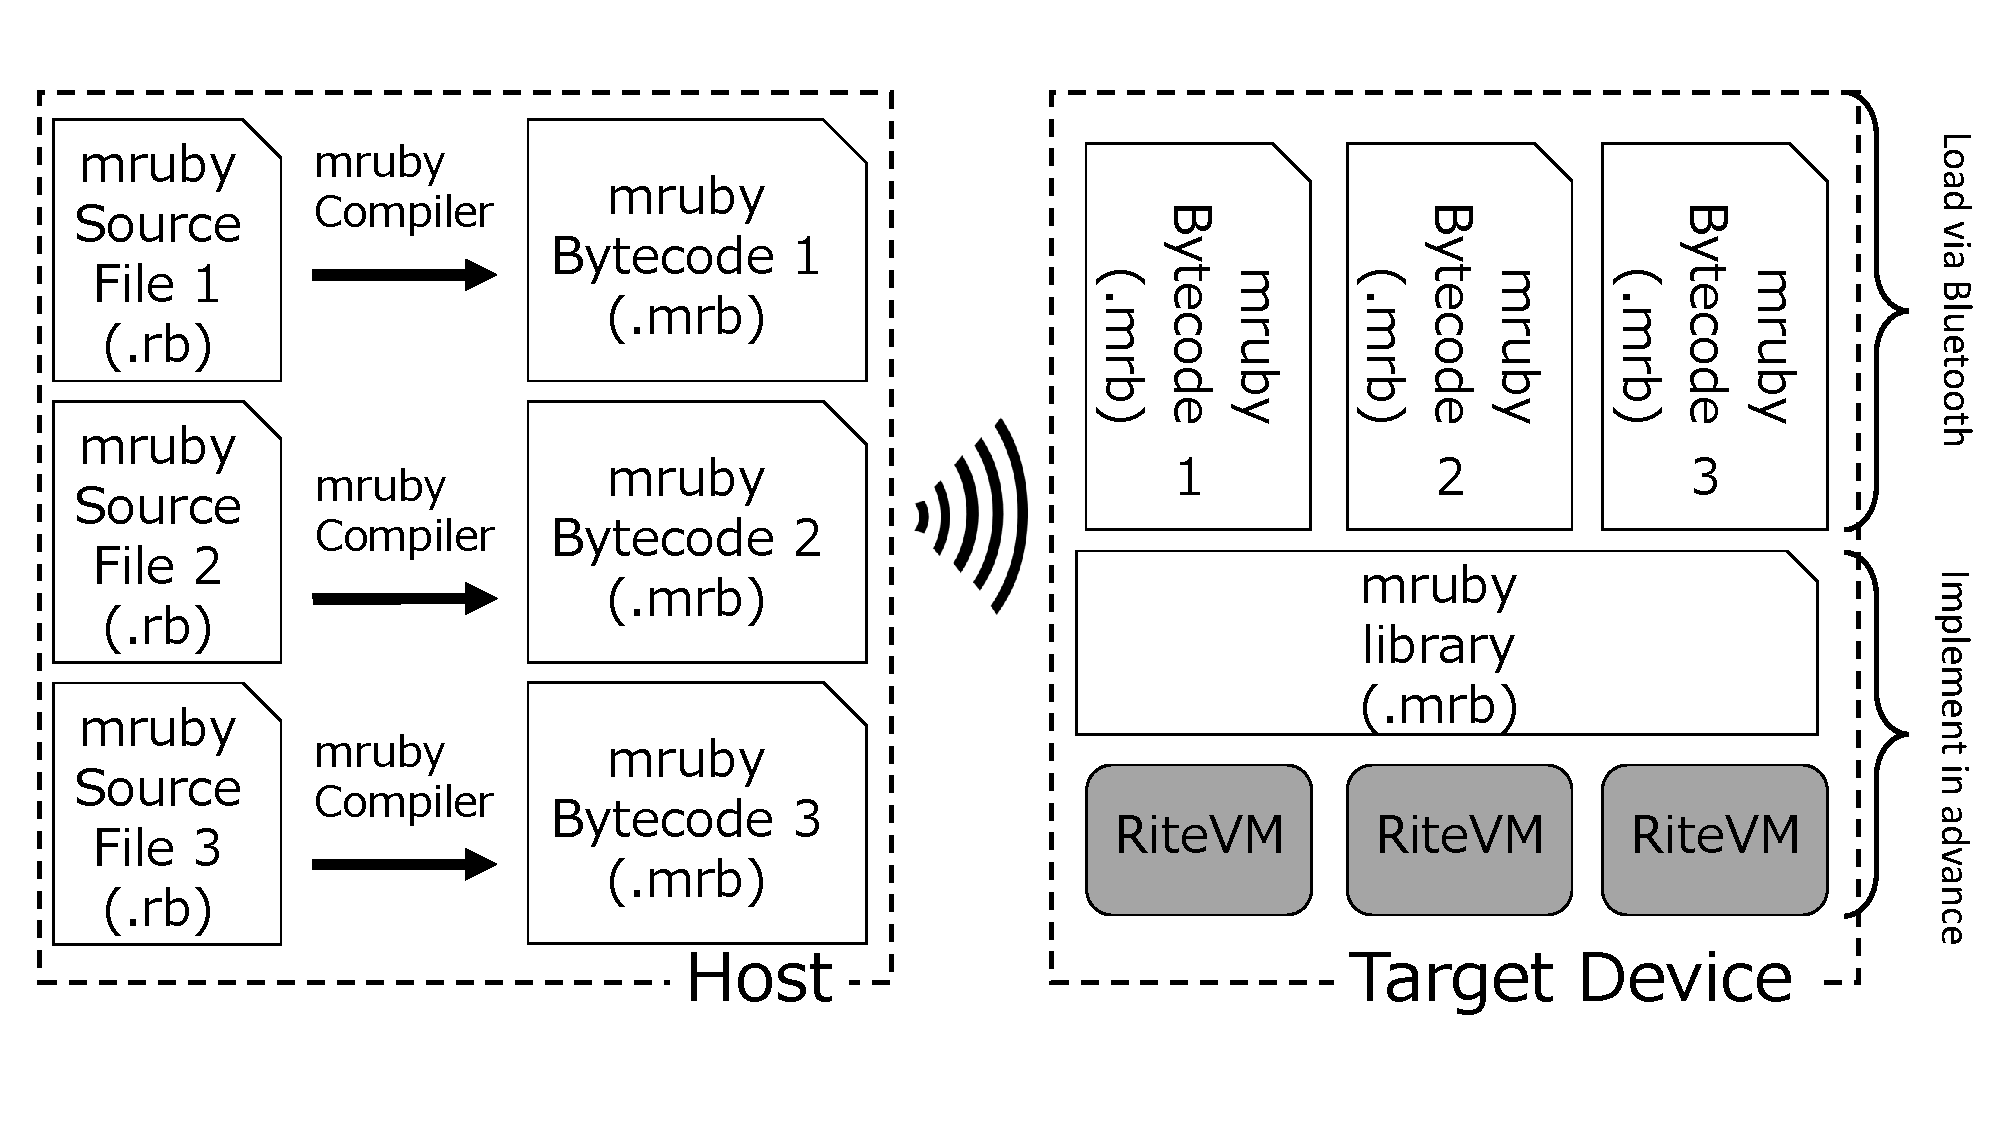
\includegraphics[width=8cm,clip]{figure/proposed.pdf}
    \caption{System Model}
    \label{fig:proposed}
\end{figure}

This section describes mruby on TECS on which the proposed framework is based.
mruby on TECS is a component-based framework for running script programs.
In mruby on TECS, two technologies are integrated: mruby and TECS.
To explain the system, mruby and TECS are also respectively described in this section.

\subsection{mruby}
\label{sec:mruby}
mruby is the light-weight implementation of Ruby programming language complying to part of the ISO standard.

Ruby is a object-oriented script language \cite{url:Ruby}.
As the main feature, Ruby is easy-to-use and easy-to-read due to its simple grammar.
Ruby can run a program with fewer code lines than C language.
Ruby improves the productivity of a software development owing to not only simple grammar also object-oriented functions such as classes and methods, exceptions, and garbage collection.

mruby is suitable for embedded systems because of faster execution with less amount of resources and takes over the usability and readability of Ruby.
In addition, VM (Virtual Machine) mechanism is used in mruby, so mruby programs can run on any operating system as long as VM is implemented.
RiteVM is a VM in mruby, that runs mruby programs.
The RiteVM mechanism is shown in Figure \ref{fig:mruby}.
The mruby compiler translates an mruby code into a bytecode, which is an intermediate code that can be interpreted by RiteVM.
The bytecodes can run on a Rite VM, and thus mruby programs can be executed on any target devices if only RiteVMs are implemented.
\begin{figure}[t]
    \centering
    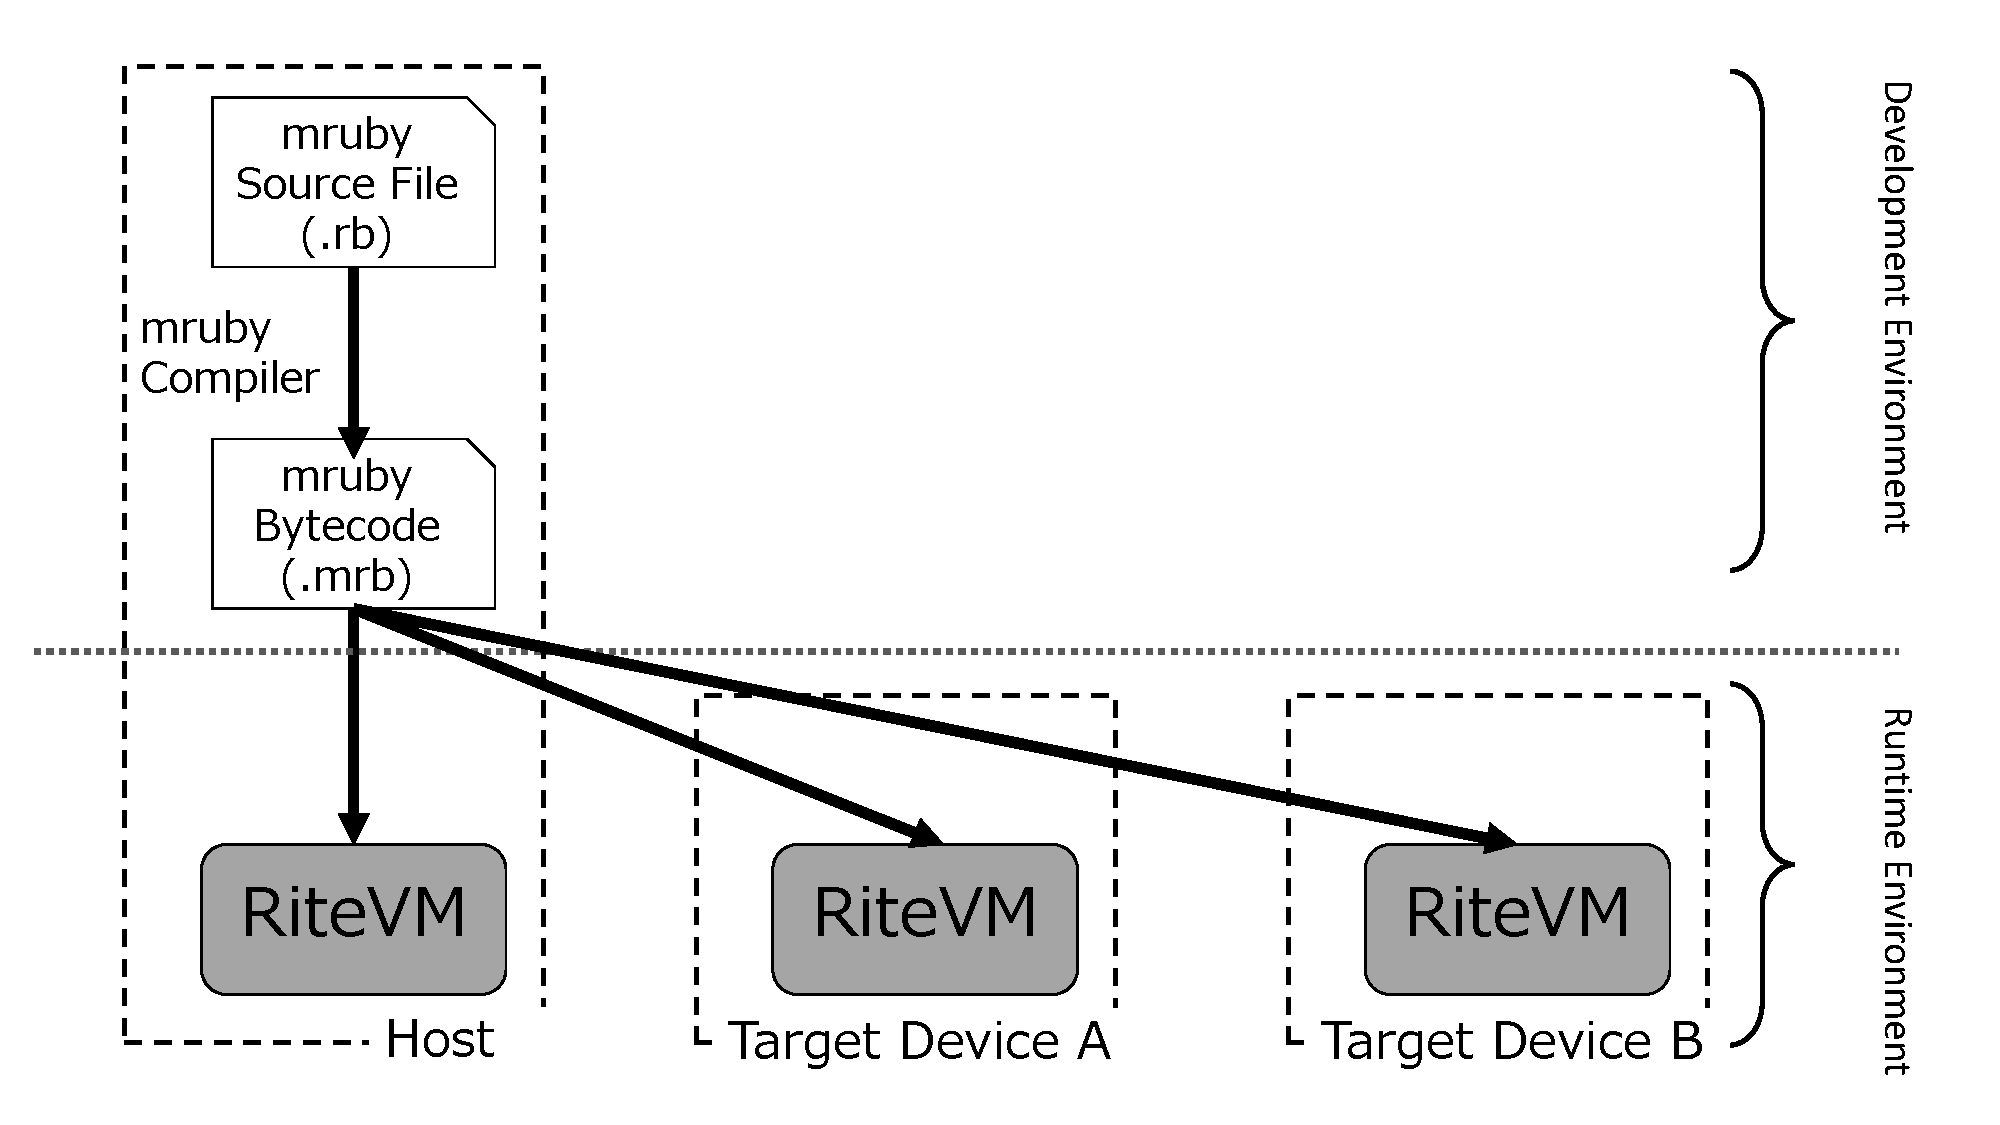
\includegraphics[width=8cm,clip]{figure/mruby.pdf}
    \caption{Mechanism of mruby/RiteVM}
    \label{fig:mruby}
\end{figure}

\subsection{TECS}
\label{sec:TECS}
TECS (TOPPERS Embedded Component System) is a component system suitable for embedded systems.
TECS helps decrease the complexity and difficulty because the generated component diagram can visualize the structure of whole software.
It can also help increase the productivity and reduce development duplication  because a common part of software is regarded as a component.

The component deployment and composition in TECS are statically performed, which gives optimization.
As a result, the overhead of execution time and memory consumption can be reduced.
There are other features of TECS, implementation in C language, source level portability, fine-grained component, etc.

\subsubsection{Component Model}\mbox{}\\

Figure \ref{fig:component} shows a component diagram.
A {\it cell} which is an instance of a component in TECS consists of {\it entry} ports, {\it call} ports, attributes and internal variables.
A {\it entry} port is an interface to provide functions with other {\it cell}s, and a {\it call} port is an interface to use functions of other {\it cell}s.
A {\it cell} has one or more {\it entry} ports and {\it call} ports.
Functions of a {\it cell} are implemented in the C language.

A type of a {\it entry}/{\it call} port is defined by a {\it signature} which is a set of functions.
A {\it signature} is the interface definition of a {\it cell}.
The {\it call} port of a {\it cell} can be connected to the {\it entry} port of another {\it cell} with the same {\it signature}.
A {\it celltype} is the definition of a {\it cell}.
{\it Celltype} defines one or more {\it call}/{\it entry} ports, attributes and internal variables.

\begin{figure}[t]
    \centering
    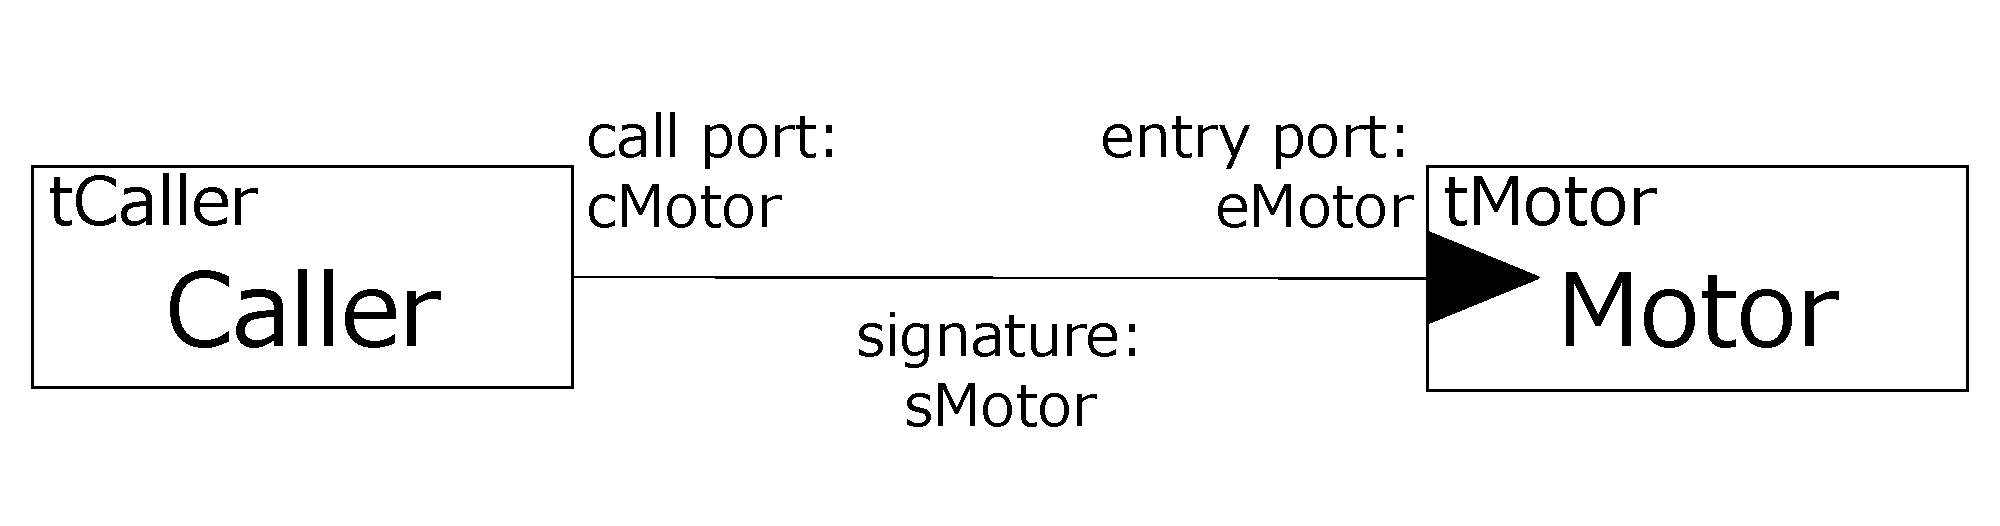
\includegraphics[width=8cm,clip]{figure/component_diagram.pdf}
    \caption{Component Diagram}
    \label{fig:component}
\end{figure}

\subsubsection{Component Description}\mbox{}\\

The description of a component in TECS is divided into three parts, {\it signature}, {\it celltype}, and build description.
TECS code is written in .cdl (component description language) file.
The component description is mentioned with an example shown in Figure \ref{fig:component} as follow.

\begin{description}
    \item[{\bf Signature Description}]\mbox{}\\
        The {\it signature} description defines an interface of a {\it cell}.
        A {\it signature} name is described following the keyword {\it signature}.
        It also has the prefix ``s".
        In this way, a {\it signature} is defined such as sMotor shown in Figure \ref{signature}.
        To make the definition of an interface clear, specifiers such as in and out are used in TECS.
        [in] and [out] represent input and output, respectively.\\
\begin{figure}[t]
\centering
\begin{lstlisting}
signature sMotor{
    int32_t getCounts(void);
    ER resetCounts(void);
    ER setPower([in]int power);
    ER stop([in] bool_t brake);
    ER rotate([in] int degrees, [in] uint32_t speed_abs,
              [in] bool_t blocking);
    void initializePort([in]int32_t type);
};
\end{lstlisting}
\caption{Signature Description}
\label{signature}
\end{figure}

    \item[{\bf Celltype Description}]\mbox{}\\
        The {\it celltype} description defines {\it entry} ports, {\it call} ports, attributes, and valuables of a {\it celltype}.
        An example of a {\it celltype} description is shown in Figure \ref{celltype}.
        A {\it celltype} name following the keyword {\it celltype} with the prefix ``t" and elements of a {\it celltype} is described.
        To define {\it entry} ports, a {\it signature} such as sMotor, and an {\it entry} port name such as eMotor follow the keyword {\it entry}.
        In the same way, {\it call} ports can be declared.
        Attributes and valuables follow the keyword attr and var respectively.\\
\begin{figure}[t]
\centering
\begin{lstlisting}
celltype tCaller{
    call sMotor cMotor;
};
celltype tMotor{
    entry sMotor eMotor;
    attr{
        int32_t attr = 100;
    };
    var{
        int32_t var;
    };
};
\end{lstlisting}
\caption{Celltype Description}
\label{celltype}
\end{figure}

    \item[{\bf Build Description}]\mbox{}\\
        The build description is used to instantiate {\it cell}s and connect {\it cell}s.
        Figure \ref{build} shows an example of a build description.
        A {\it celltype} name such as tMotor, and a {\it cell} name such as Motor follow the keyword {\it cell}.
        To compose {\it cell}s a {\it call} port, a {\it signature}, a {\it entry} port in order are described.
        In this example, a {\it entry} port eMotor in a {\it cell} Motor is connected to a {\it call} port cMotor in a {\it cell} Caller.\\
\begin{figure}[t]
\centering
\begin{lstlisting}
cell tMotor Motor{
};
cell tCaller Caller{
    cMotor = Motor.eMotor;
};
\end{lstlisting}
\caption{Build Description}
\label{build}
\end{figure}

\end{description}

\subsection{mruby on TECS}
\label{sec:mruby on TECS}
mruby on TECS is a component-based framework for running script language.
This framework uses two technologies, mruby and TECS.

\subsubsection{System Model}\mbox{}\\

The system model of mruby on TECS is shown in Figure \ref{fig:system_model}.
Each mruby program, which is bytecode, runs on its own RiteVM as a componentized task of an RTOS.
TECS components support various embedded drivers such as motor and sensor drivers.

An mruby-TECS bridge plays a role to call a native program (e.g.,C legacy code) from an mruby program.
The mruby-TECS bridge provides native libraries for mruby.
It also gives TECS components to receive the invocation from an mruby program.
The mruby-TECS bridge is described in more detail bellow.

As the target RTOS, TOPPERS/HRP2 \cite{url:HRP2}, \cite{par:hr-tecs} is used in this paper.
TOPPERS/HRP2 is an RTOS based on $\mu$ITRON with memory protection.
However, mruby on TECS does not depend on the RTOS because TECS supports not only TOPPERS/HRP2 but also the other RTOSs such as OSEK \cite{par:OSEK} and TOPPERS/ASP \cite{url:ASP}.

\begin{figure}[t]
    \centering
    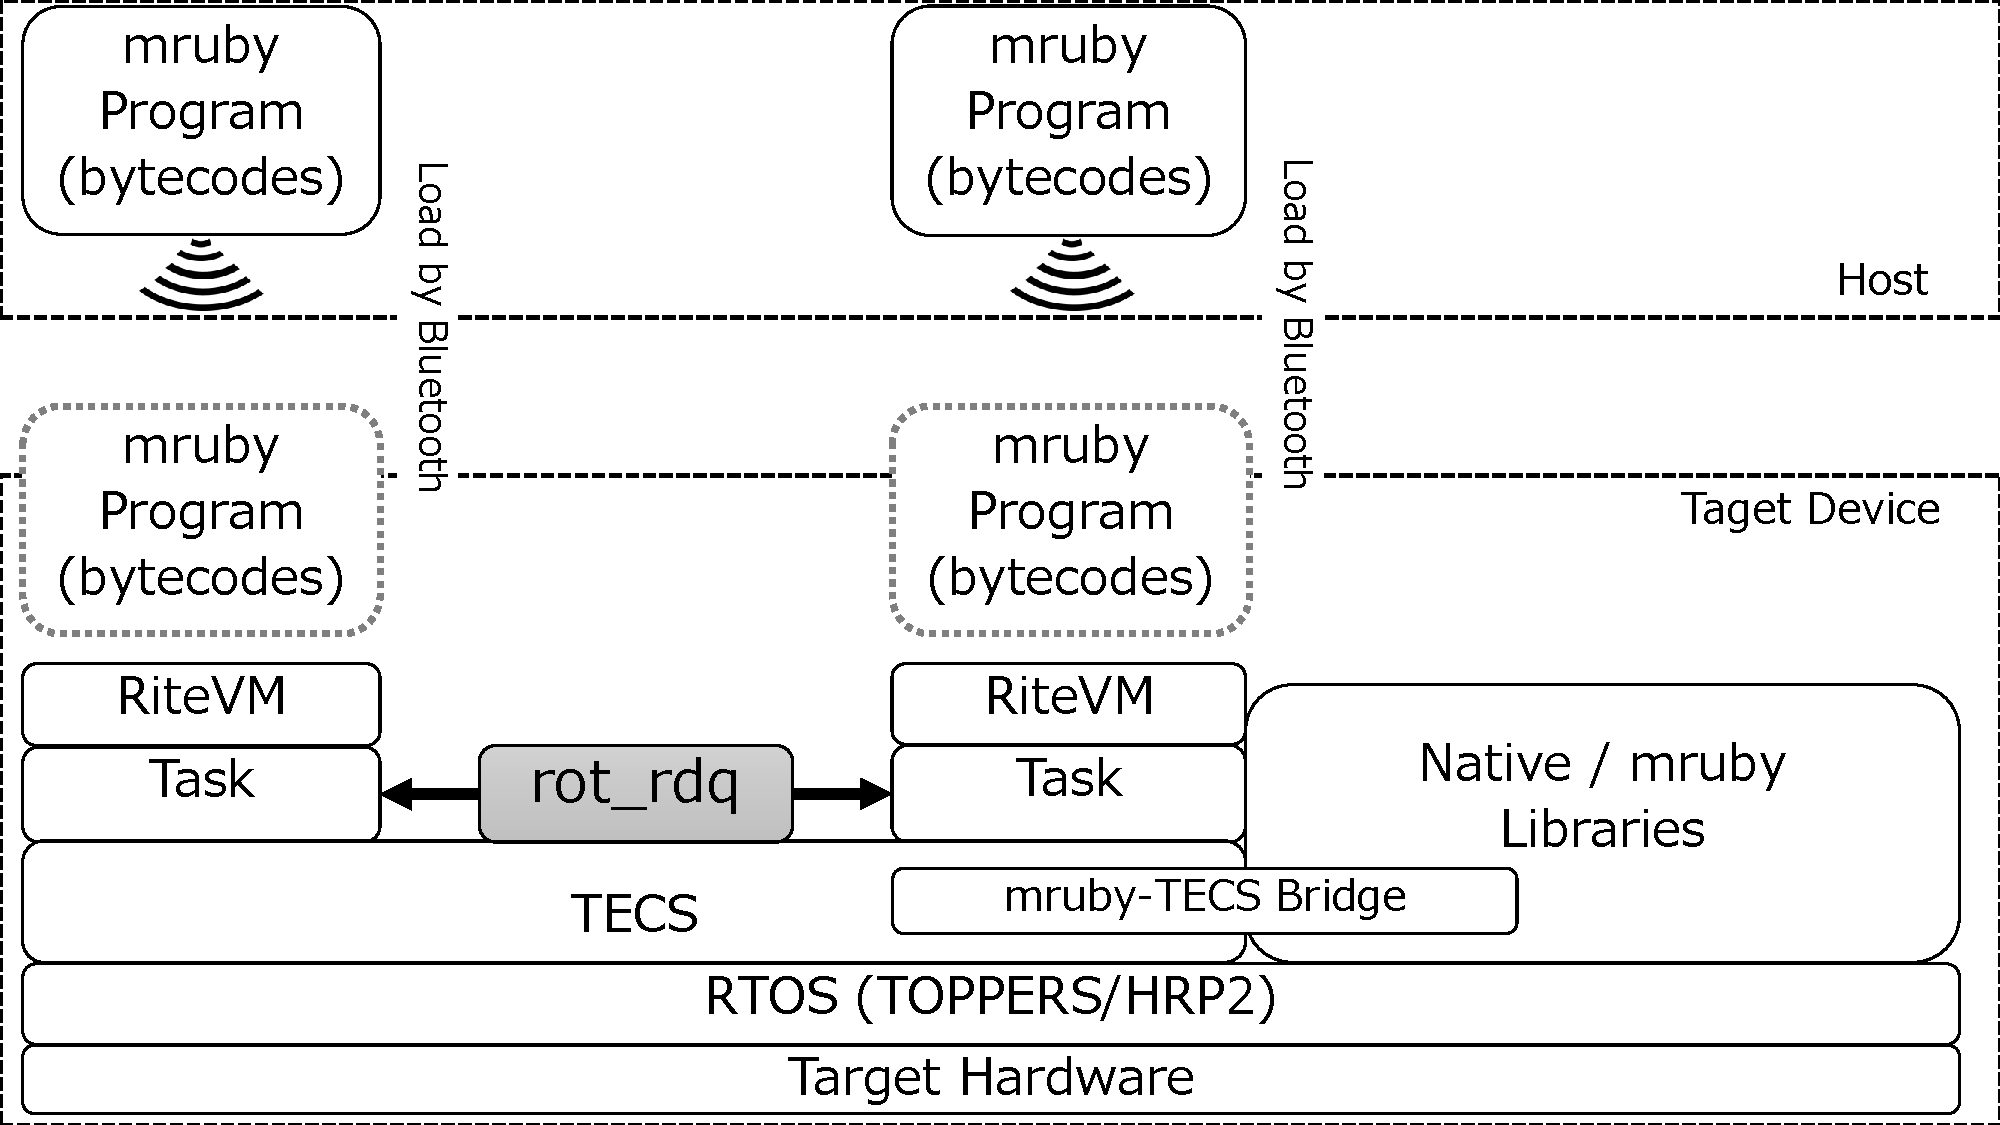
\includegraphics[width=8cm,clip]{figure/system_model.pdf}
    \caption{System Model}
    \label{fig:system_model}
\end{figure}

\subsubsection{mruby-TECS Bridge}\mbox{}\\

There is a great difference between the execution time of mruby and C language.
According to  \cite{par:mrubyonTECS}, mruby programs are several hundreds times slower than C programs.
The execution of mruby bytecode on a RiteVM is not as efficient as that of C language.
Thus it is difficult to use mruby for all of code.

The use of Ruby on embedded devices provides the benefit of productivity and maintainability due to the ease to use and read.
On the other hands, it is necessary to implement parts of applications in C language in order to manipulate actuators and sensors, and also make a critical section of code run quickly.

Figure \ref{fig:mruby_TECS_bridge} shows an example of use of an mruby-TECS bridge for controlling a motor.
The left side of BridgeMotor belongs to the mruby program.
The right side of BridgeMotor belongs to TECS component.
\begin{figure}[t]
    \centering
    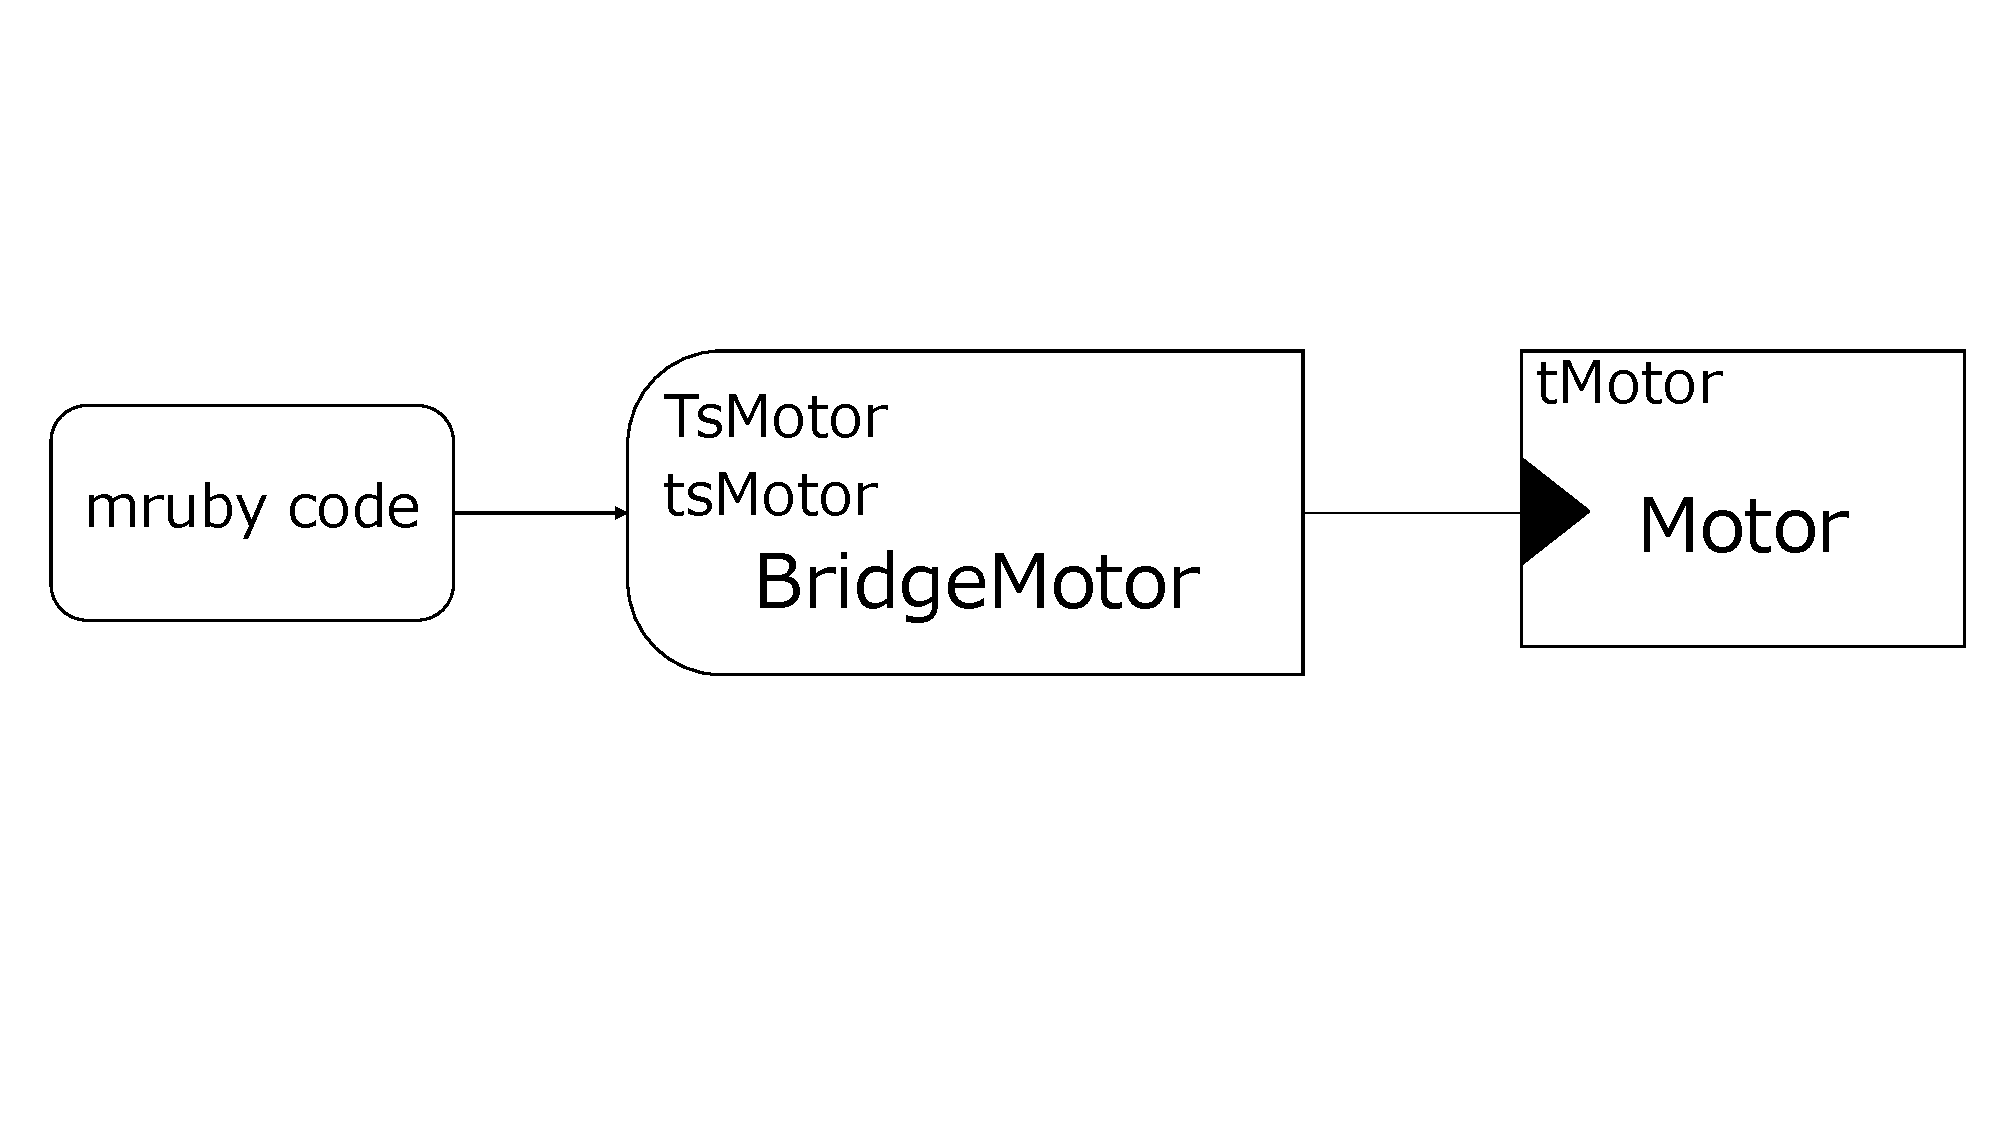
\includegraphics[width=8cm,clip]{figure/mruby_TECS_bridge.pdf}
    \caption{mruby-TECS Bridge}
    \label{fig:mruby_TECS_bridge}
\end{figure}

The mruby-TECS bridge generates two things.
One is a {\it celltype} to receive invocation from the mruby program.
The other thing is an mruby class that corresponds to the TECS component specified by the developers to invoke a C function from the mruby program.

A code of an mruby-TECS bridge is generated.
The generation code supports registration of classes and methods for mruby.
The methods in an mruby class are defined by generation codes for an mruby-TECS bridge, such as setPower and stop.
Thus, when a method is called in an mruby program, an mruby-TECS bridge calls the function defined in the TECS component such as a Motor {\it cell}.


\section{mruby Bytecode Loader Using Bluetooth}
\label{sec:mruby bytecode loader using Bluetooth}
This section describes an additional function of mruby on TECS, mruby bytecode loader using Bluetooth.
In the current system, all binary data including bytecodes are in an SD card.
Developers must insert and pull out the SD card every time the source program are modified.
It causes a low work efficiency that such a work must be repeated.
mruby bytecode loader using Bluetooth makes the developers' burden decrease.
The work that an SD card is in and out needs to be done just once in the beginning.

The development flow in mruby bytecode loader using Bluetooth is shown in Figure \ref{fig:bluetooth_loader}.
The RiteVM and mruby library are compiled and copied in the SD card at the first.
These are assumed not to be modified.
The binary data transferred with Bluetooth is the bytecode of the main source.
In the host, the source files (.rb) are edited and compiled into the bytecodes (.mrb) by an mruby compiler.
The generated bytecodes are transferred from the host to the target device with Bluetooth.

\begin{figure}[t]
    \centering
    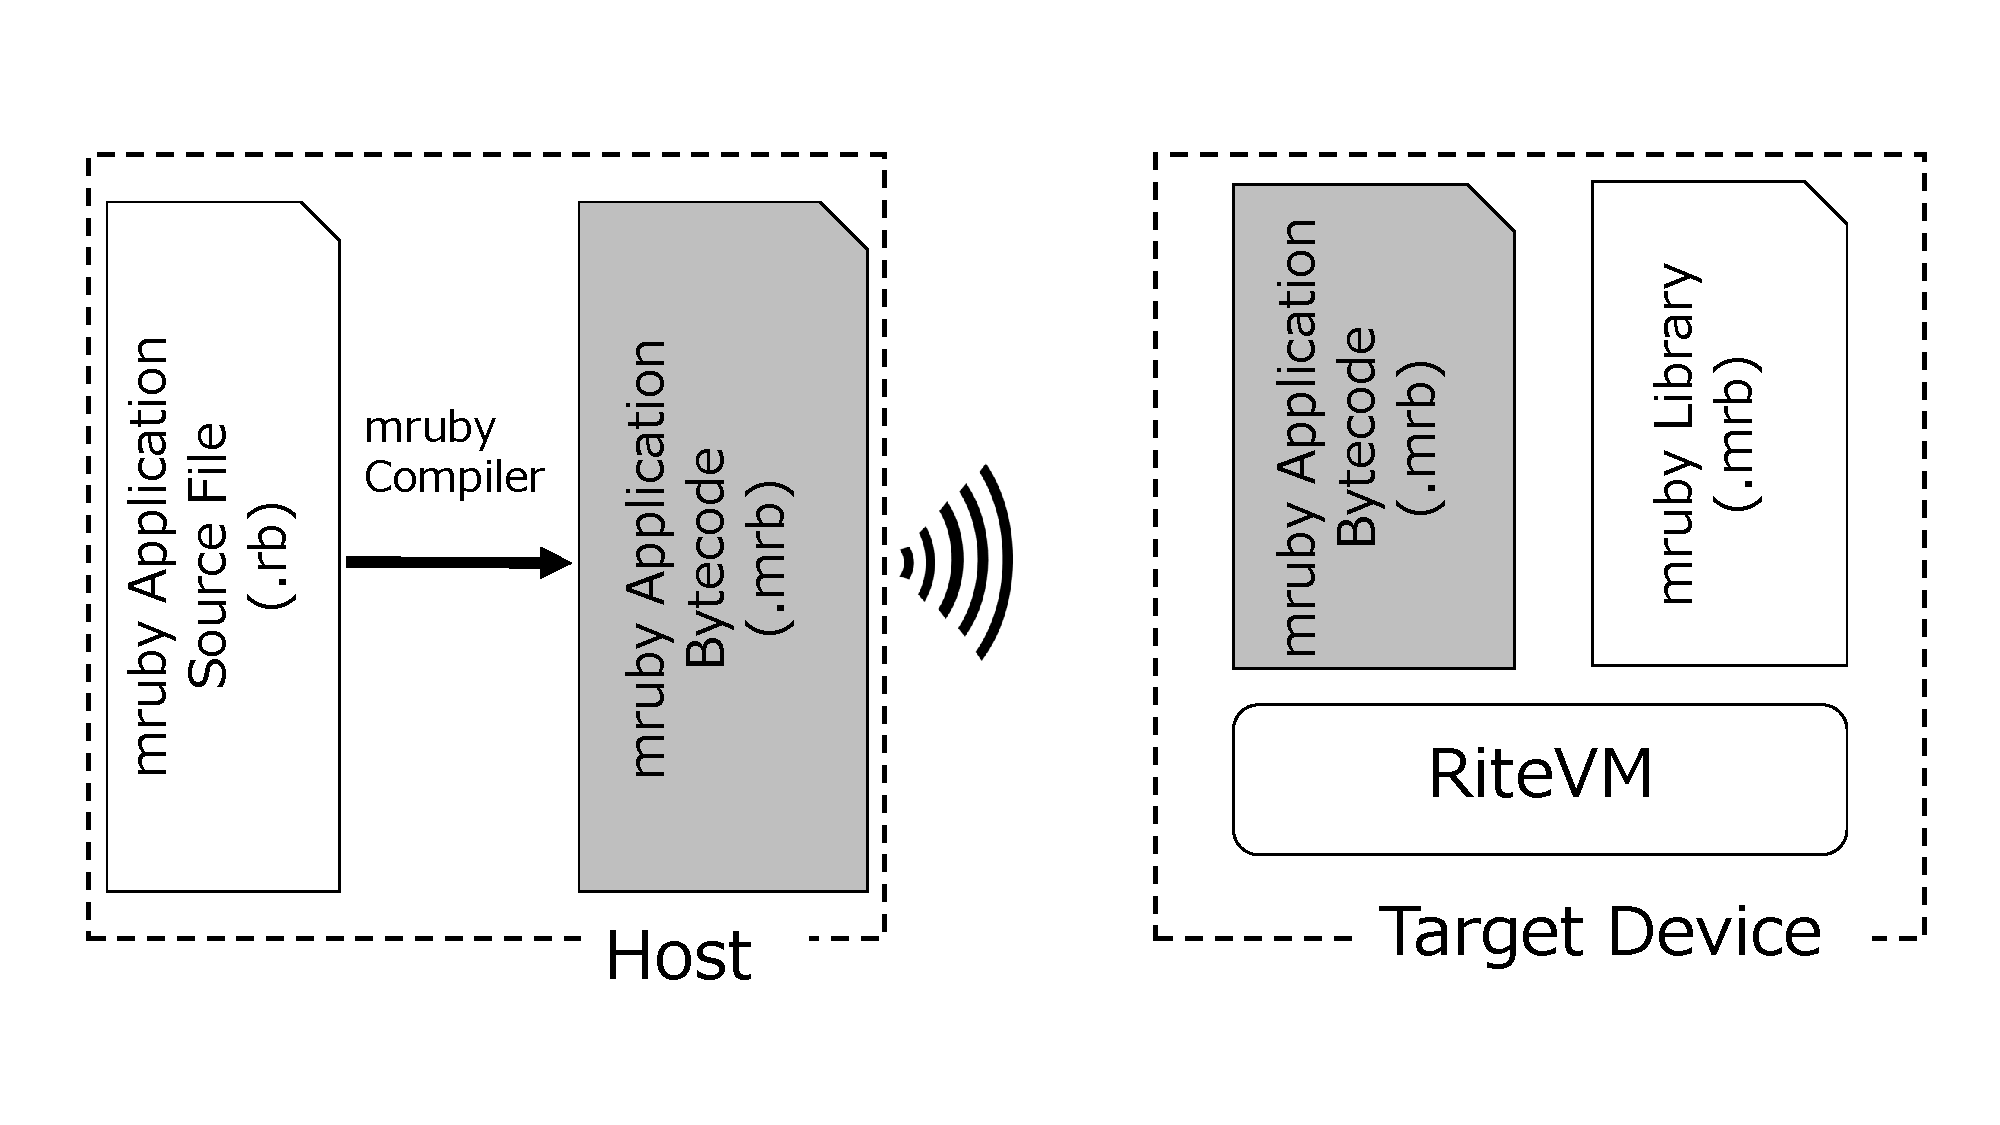
\includegraphics[width=8cm,clip]{figure/bluetooth_loader.pdf}
    \caption{Development Flow in mruby bytecode loader using Bluetooth}
    \label{fig:bluetooth_loader}
\end{figure}

\subsection{Component of mruby bytecode loader using Bluetooth}
The proposed framework provides components of mruby bytecode loader using Bluetooth to use the function.
A component of mruby bytecode loader using Bluetooth is an extension of the RiteVM component, which is described in \cite{par:mrubyonTECS}.
The component plays a role in receiving bytecodes via Bluetooth, and also manages RiteVM configuration such as automatically generates the bytecode in the build description.
This generated bytecode is prepared beforehand in the SD card such as mruby libraries, and different from a bytecode transferred with Bluetooth.

Figure \ref{fig:component_bluetooth} shows a component diagram of MrubyTask1 and MrubyBluetooth1 {\it cell}s.
The MrubyTask1 {\it cell} is a componentized task of the RTOS (TOPPERS/HRP2).
TOPPERS/HRP2 is described in \cite{url:HRP2}, \cite{par:ht-tecs}.
The MrubyBluetooth1 is a component of mruby bytecode loader using Bluetooth.
A bytecode which is a compiled mruby program in the host is transferred and received at the top of the mruby bytecode loader using Bluetooth component.
In this framework, ZMODEM \cite{par:zmodem} is used as a binary transfer protocol.

\begin{figure}[t]
    \centering
    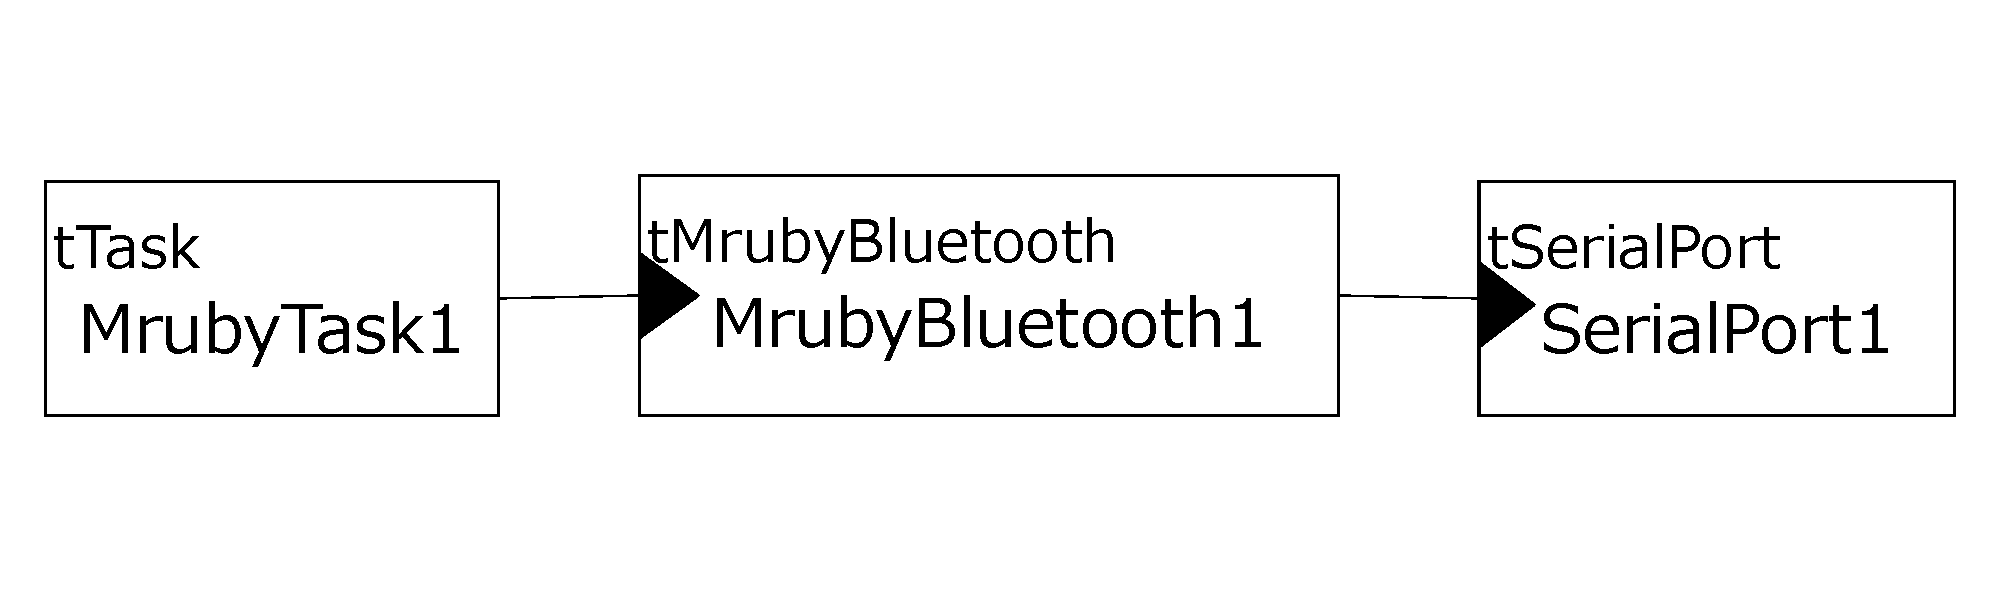
\includegraphics[width=8cm,clip]{figure/component_bluetooth.pdf}
    \caption{Component Diagram of mruby bytecode loader using Bluetooth}
    \label{fig:component_bluetooth}
\end{figure}

Figure \ref{fig:control_flow} shows the process of executing mruby program in a component of mruby bytecode loader using Bluetooth, which is like MrubyBluetooth1.
First, a pointer of {\it mrb\_state} structure is initialized.
{\it mrb\_state} is a set of states and global variables used in mruby.
Second, the bytecode of mruby libraries is read.
mruby libraries are a set of Ruby classes such as motor class and sensor class.
For example, motor class defines methods to rotate and stop a motor.
The tMrubyBluetooth {\it cell} has two attributes as shown in Figure \ref{celltype_mrubybluetooth}: {\it mrubyFile} and {\it irep}.
The {\it mrubyFile} indicates the program files of mruby libraries.
{\it [omit]} is only used for the TECS generator, thus the attribute, {\it mrubyFile}, does not consume memory.
The irep is the pointer of the array stored the bytecode of mruby libraries.
In short the bytecode of mruby libraries is stored as an attribute of the component when compiling for the first time.
Third, the bytecode of the mruby program transferred with Bluetooth is read .
The bytecode transmitted via Bluetooth is stored in an array of type uint8\_t, which is the same as type char.
The array is different from that of holding the mruby library bytecode.
Two bytecodes are read separately in the {\it mrb\_state}.
Finally, an mruby task runs.
When the mruby program is modified, only the bytecode of the modified program should be transferred.
mruby libraries need not be touched because libraries are not normally changed.
The concrete main code of tMrubyBluetooth is shown in Figure \ref{maincode_mrubybluetooth}.
\begin{figure}[t]
    \centering
    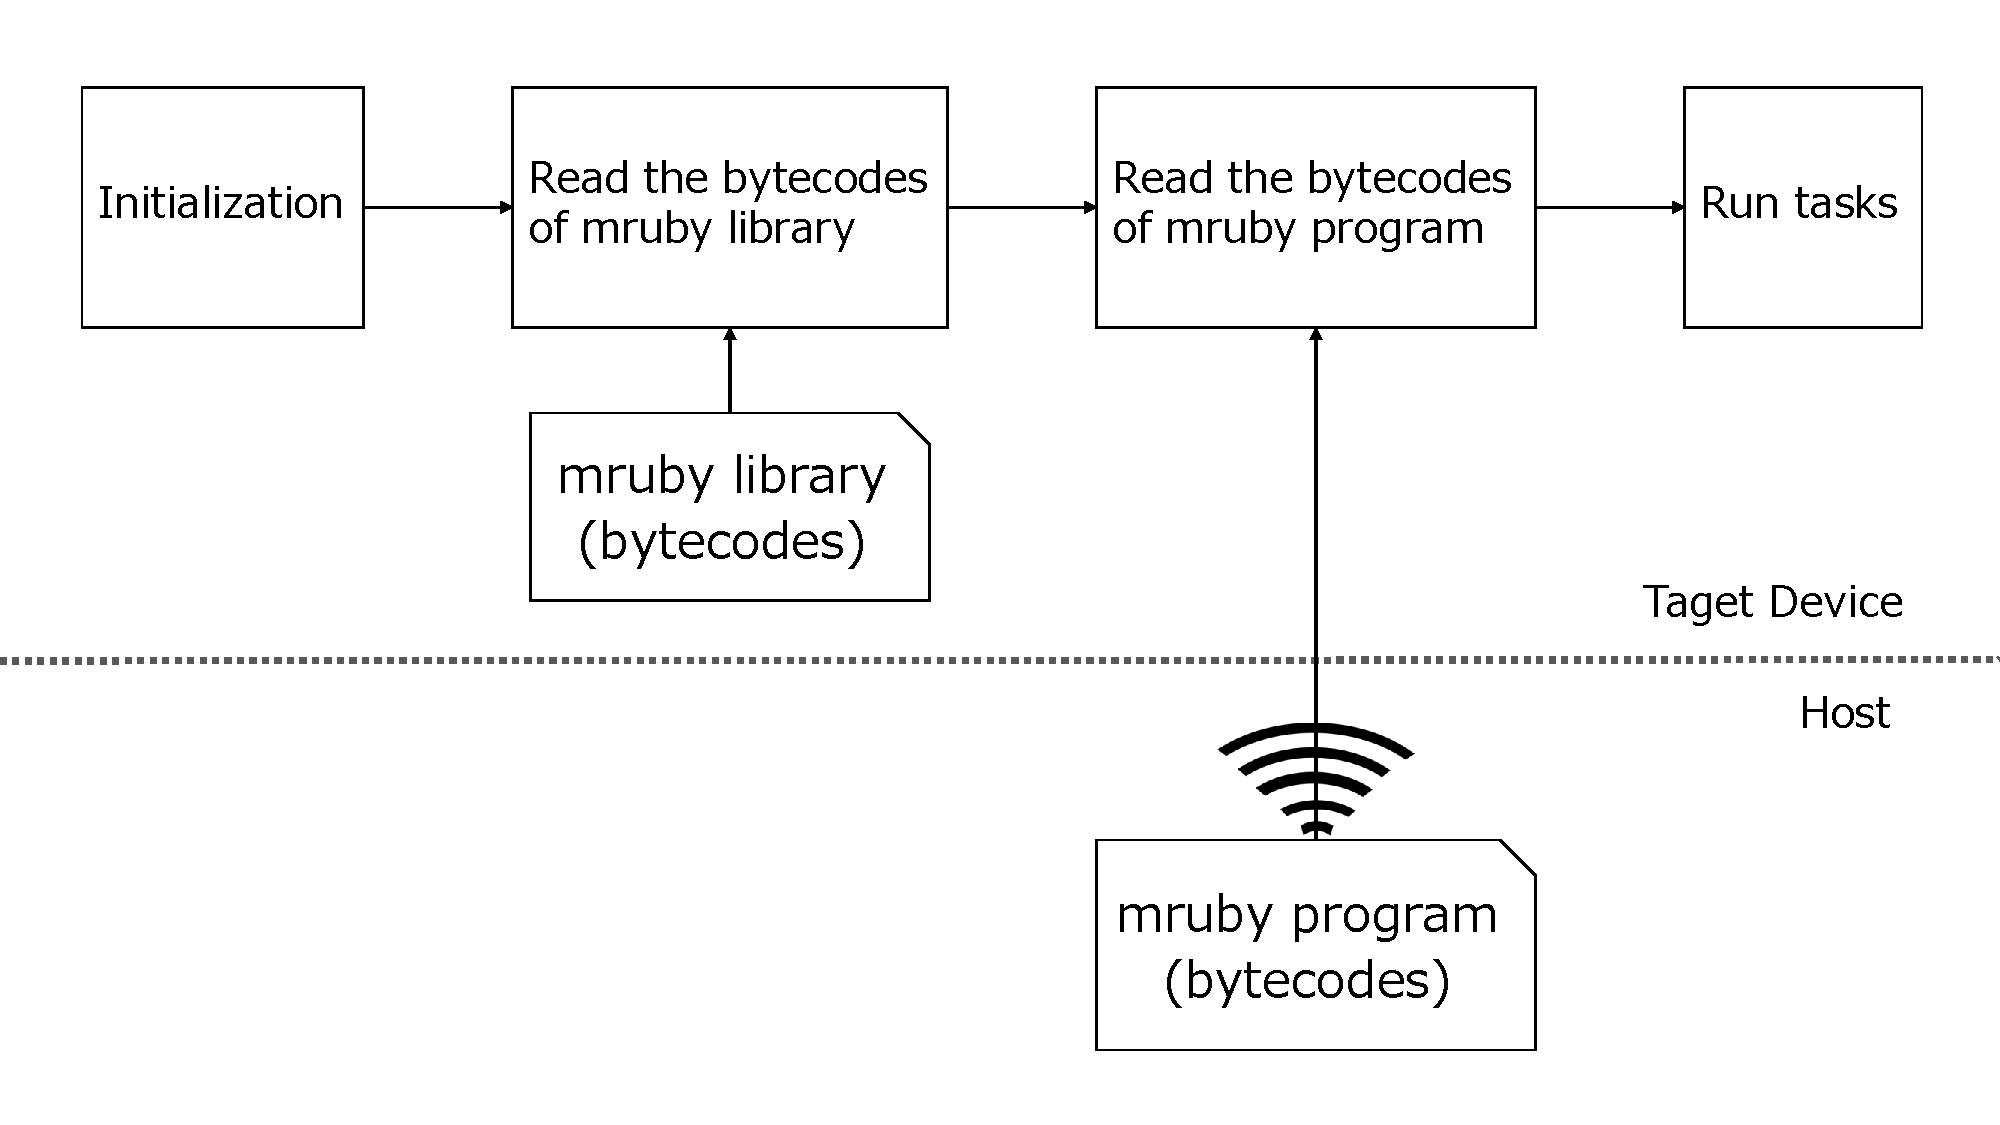
\includegraphics[width=8cm,clip]{figure/control_flow.pdf}
    \caption{Control Flow of mruby bytecode loader using Bluetooth}
    \label{fig:control_flow}
\end{figure}
\begin{figure}[t]
\centering
\begin{lstlisting}
celltype tMrubyBluetooth{
    entry sTaskBody eMrubyBody;
    attr{
      [omit]char_t *mrubyFile;
      char_t *irepLib=C_EXP("&$cell_global$_irep");
      uint8_t irepApp[COUNT_STK_T(TMAX_APP_BINARY_SIZE)]
              __attribute__((nocommon));
    };
};
\end{lstlisting}
\caption{Celltype Description for mruby bytecode loader using Bluetooth}
\label{celltype_mrubybluetooth}
\end{figure}

\begin{figure}[t]
\centering
\begin{lstlisting}
void
eMrubyBody_main(CELLIDX idx)
{
  /* Declaration variables */
  mrb_state *mrb;
  mrbc_context *c;
  /* New interpreter instance */
  mrb = mrb_open();
  // Omit: error check for mrb_state
  /* New mruby context */
  c = mrbc_context_new(mrb);
  // Omit: initialization of mruby-TECS bridge
  /* Receive the bytecode via Bluetooth */
  bluetooth_loader( ATTR_app );
  /* Load mruby library bytecode and run */
  mrb_load_irep_cxt(mrb, ATTR_lib, c);
  /* Load mruby application bytecode and run */
  mrb_load_irep_cxt(mrb, ATTR_app, c);
  if (mrb->exc) {
    /* Failure to execute */
    mrb_p(mrb, mrb_obj_value(mrb->exc));
    exit(0);
  }
  /* Free mruby context */
  mrbc_context_free(mrb, c);
  /* Free interpreter instance */
  mrb_close(mrb);
}

\end{lstlisting}
\caption{Main code for mruby bytecode loader using Bluetooth}
\label{maincode_mrubybluetooth}
\end{figure}
\section{Multitask}
\label{sec:Multitask}
This section describes implementation of multitasking in the proposed framework.
mruby on TECS has supported multitasking.
However, multitask processing in mruby on TECS requires the knowledge of the RTOS (TOPPERS/HRP2) for developers.
One of approaches for multitasking is co-routine.
Co-routine is scheduled by developers with the functions such as {\it resume} and {\it yield}, and thus co-routine does not receive the OS's support.
Besides, as another method, {\it delay}, a service call of $\mu$ITRON, can be used for multitasking, but developers have to schedule as the same as co-routine.
In the proposed framework, as an approach for multitask processing, {\it rotateReadyQueue}, a service call of $\mu$ITRON, is implemented.
A cyclic handler calls {\it rotateReadyQueue} that switches tasks, which enables developers to develop applications without concern for multitasking.

\subsection{rotateReadyQueue}
The case is assumed that there are two tasks with the same priority, and both tasks are in an infinite loop.
In the current system, when one task is executed first, another task would not be executed.
That is because the task with first execution runs in the loop.

When {\it rotateReadyQueue} is called, tasks with the same priority are switched as shown in Figure \ref{fig:rotateReadyQueue}.
The argument of {\it rotateReadyQueue} is the priority.

The {\it rotateReadyQueue} can be performed if the number of tasks is more than two.
For example, three tasks are in the order: task 1, 2, and 3.
In this case, the order is changed, task 2, 3 and, 1, when the {\it rotateReadyQueue} is called.

\begin{figure}[t]
    \centering
    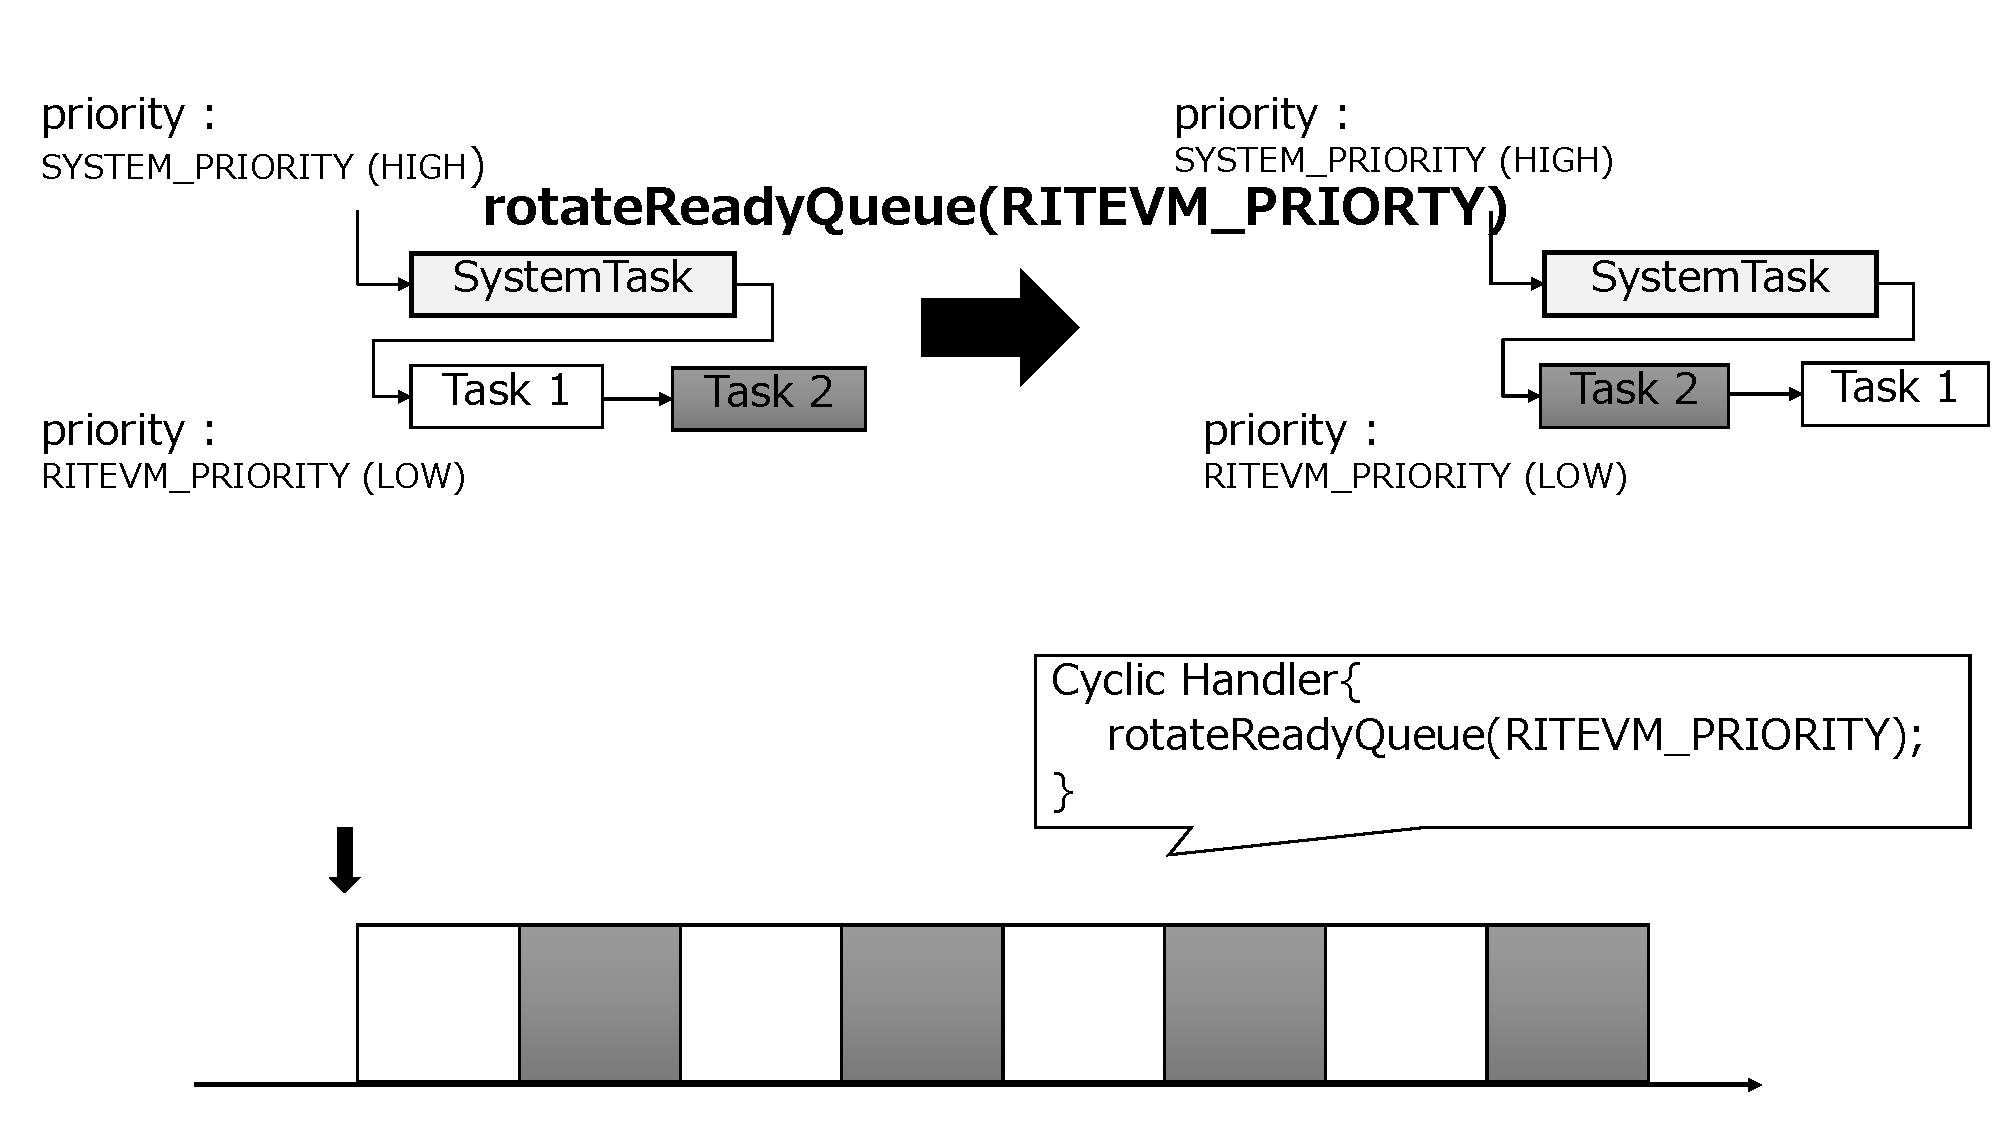
\includegraphics[width=8cm,clip]{figure/rotateReadyQueue.pdf}
    \caption{rotateReadyQueue}
    \label{fig:rotateReadyQueue}
\end{figure}

\subsection{Component of Cyclic Handler}
Figure \ref{fig:cyclic_handler} shows a component diagram of the cyclic handler.
The components of cyclic handler consist of two components: CyclicHandler and CyclicMain.
CyclicHandler {\it cell} configures the cyclic handler based on ITRON.
Cyclic handlers based on ITRON are described in detail \cite{par:microITRON}.
The cyclic handler has five arguments: ID, attribute, cyclic time, cyclic phase and access pattern.
CyclicHandler {\it cell} has these arguments as attributes of the {\it cell}.
CyclicMain {\it cell} is a component to perform the processing body of a cyclic handler.
{\it rotateReadyQueue} is implemented as the body.
Figure \ref{celltype_cyclic_handler} shows tCyclicMain {\it celltype}, which has a {\it call} port, an {\it entry} port and an attribute.
The {\it call} port is connected with the {\it entry} port of the Kernel {\it cell} ({\it tkernel.eiKernel}) to call functions of the kernel. 
The attribute is used as an arguments of {\it rotateReadyQueue}.

Figure \ref{build_cyclic_handler} shows a build description that corresponds to the component diagram shown in Figure \ref{fig:cyclic_handler}.
In the part of CyclicHandler {\it cell}, configurations of a cyclic handler is described such as attribute, cyclicTime and cyclicPhase.
In this case, the cyclic handler is executed when it is generated because the attribute is {\it TA\_STA}.
The cyclic handler is executed every one msec.
In another part, the priority of CyclicMain {\it cell} is described.
EV3\_MRUBY\_VM\_PRIORITY defines the priority of mruby tasks.
In the main of CyclicMain, {\it rotateReadyQueue} is implemented and the priority is passed as the argument.
If developers do not need the cyclic handler, the .cdl files shown as Figures \ref{celltype_cyclic_handler} and \ref{build_cyclic_handler} should be commented out such as {\it //import($<$**.cdl$>$);}.
This ease comes from component-based development with TECS.

\begin{figure}[t]
    \centering
    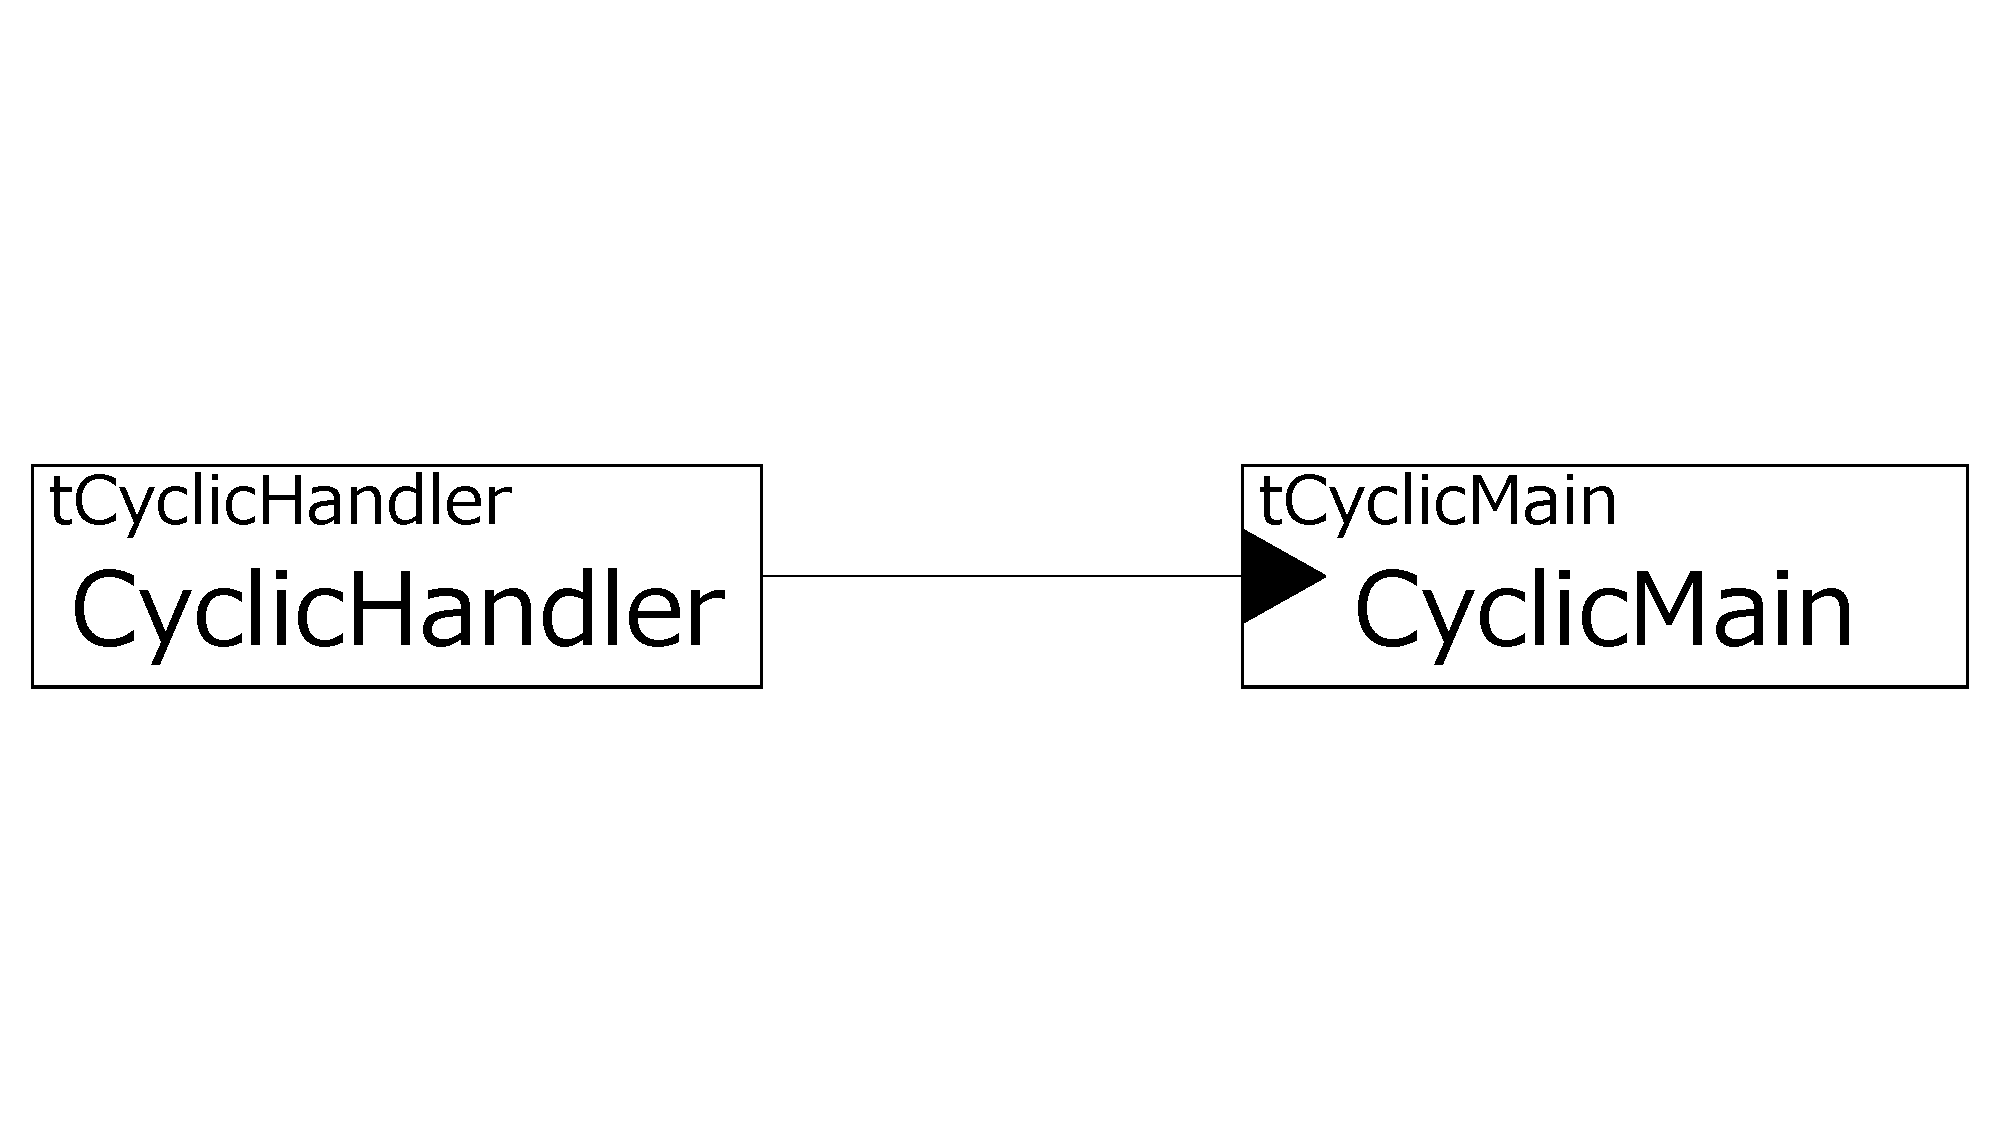
\includegraphics[width=8cm,clip]{figure/cyclic_handler.pdf}
    \caption{Component Diagram of Cyclic Handler}
    \label{fig:cyclic_handler}
\end{figure}
\begin{figure}[t]
    \centering
    \begin{lstlisting}
celltype tCyclicHandler {
    [inline] entry sCyclic eCyclic;
    call  siHandlerBody  ciBody;
    attr {
    	[omit] ATR    attribute = C_EXP("TA_NULL");
    	[omit] RELTIM cyclicTime;
    	[omit] RELTIM cyclicPhase = 0;
    };
};
celltype tCyclicMain{
    require tKernel.eiKernel;
    entry siHandlerBody eiBody;
    attr {
        PRI priority;
    };
};
    \end{lstlisting}
    \caption{Celltype Description of Cyclic Handler}
    \label{celltype_cyclic_handler}
\end{figure}
\begin{figure}[t]
    \centering
    \begin{lstlisting}
cell tCyclicHandler CyclicHandler{
    ciBody = CyclicMain.eiBody;
    attribute = C_EXP("TA_STA");
    cyclicTime = 1;
    cyclicPhase = 1;
};
cell tCyclicMain CyclicMain{
    priority =
        C_EXP("RITEVM_PRIORITY");
};
   \end{lstlisting}
    \caption{Build Description of Cyclic Handler}
    \label{build_cyclic_handler}
\end{figure}
 
\subsection{Synchronization of Multiple RiteVM Tasks}
In the proposed framework, RiteVMs read mruby bytecodes, and then execute the applications.
Eventflag, one of synchronous processing, is applied to synchronize the starting of multiple mruby applications.
Each task sets the flag pattern such as 0x01 (01) and 0x02 (10), and then waits the flag pattern, 0x3 (11), with AND.
This process can also apply to the case of the more tasks.
For example, in the case of the four RiteVM tasks, each task sets the flag pattern such as 0x01 (0001), 0x02 (0010), 0x04 (0100)  and 0x08 (1000), and then waits 0x0f (1111) with AND.

In the proposed framework, the set pattern and wait pattern are defined as attributes of the component as shown in Figure \ref{fig:Eventflag}.
This design such as {\it cEventflag\_set(ATTR\_setPattern)} enables the program without ``if" statements.
The components of eventflag are built with {\it [optional]} in TECS.
{\it [optional]} means that the codes are run only when the call port is connected.
The identical file can be used even if developers do not use eventflag.
In other words, it is not necessary to compile/link the different file.
These features are also advantages of component-based development.

\begin{figure}[t]
    \centering
    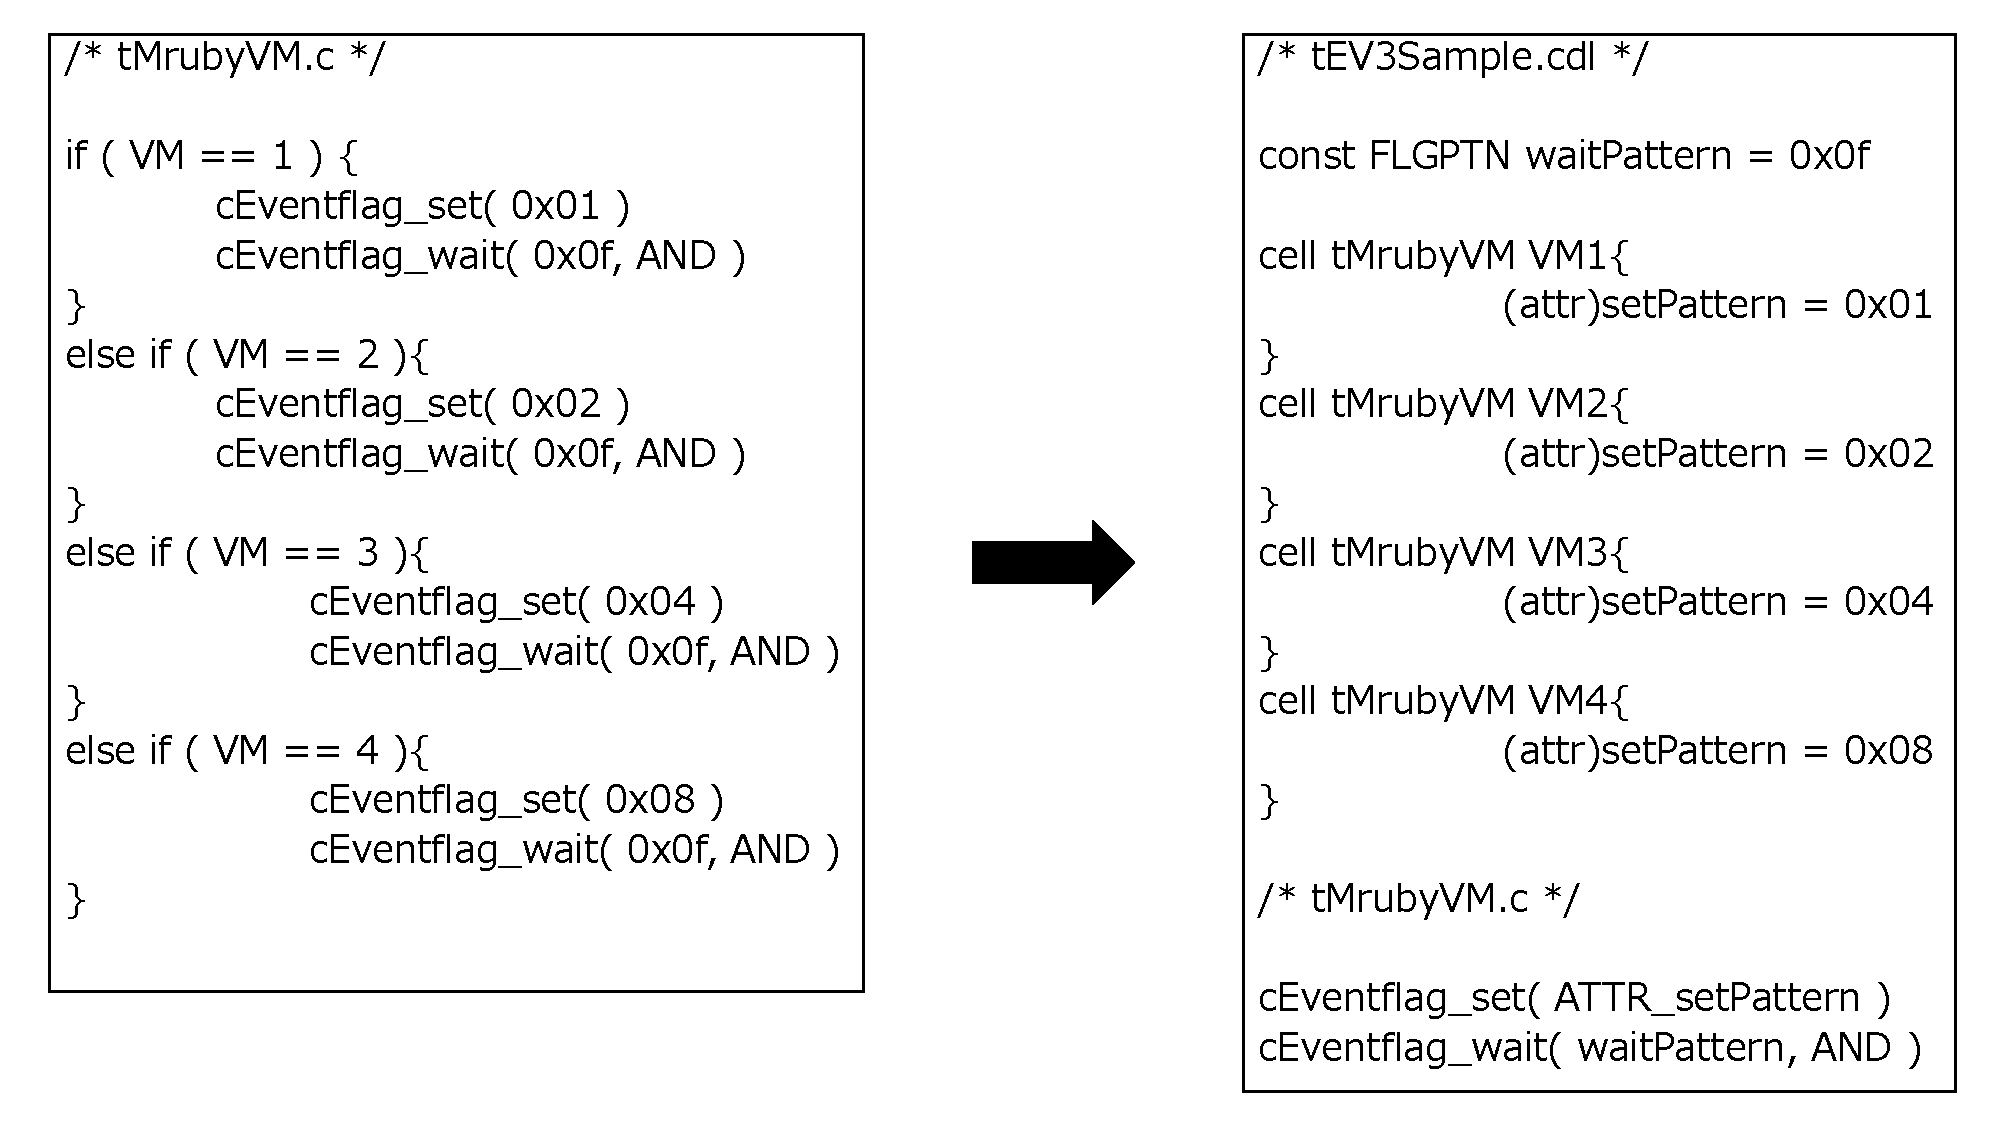
\includegraphics[width=8cm,clip]{figure/Eventflag.pdf}
    \caption{The design for Eventflag using TECS}
    \label{fig:Eventflag}
\end{figure}
 
\section{Experimental Evaluation}
\label{sec:Evaluation}
This section mentions experimental results and their consideration.
To analyze the advantages and disadvantages of the proposed framework, the evaluations are performed as follows.
\begin{itemize}
        \item the comparison of the size and transfer time between an mruby application including mruby library and not
        \item the comparison of the application execution time with singletasking, co-routine, and multitasking
        \item the comparison of the overhead for each cyclic period of calling {\it rotateReadyQueue}
\end{itemize}

This paper demonstrates the proposed system on a LEGO MINDSTORMS EV3 (300MHz ARM9-based Sitara AM1808 system-on-a-chip) compiled with gcc 4.9.3 -O2 and mruby version 1.2.0.
The 100,000 times loop program is used as mruby application for evaluation of execution time.
In detail, the singletask program loops 100,000 times, and the multitask and co-routine programs loop 50,000 times in each task.

The size and transfer time for mruby application and mruby application including library is shown in Table \ref{tab:size_and_time}.
The bytecode of mruby application including library is larger and slower than that of only mruby application in terms of size and transfer time.
In the proposed framework, developers send only mruby application and prepare mruby library in advance.
Therefore, the design can send the bytecode faster.
In addition, the design can save the time to insert an SD card.
These advantages lead to improving the work efficiency.

\begin{table}[t]
    \centering
    \caption{Comparison of the size and transfer time between an mruby application including mruby libraries and not}
    \begin{tabular}{c||c|c}
                        & mruby Application \& Library & mruby Application  \\ \hline
          Size          & 14,044 bytes                 & 199 bytes          \\ %\hline
          Transfer Time & 356.015 msec                 & 58.708 msec        \\
    \end{tabular}
    \label{tab:size_and_time}
\end{table}

The comparison of the application execution time with singletasking, co-routine, and multitasking is shown in Figure \ref{fig:comparison_s_c_m}.
In Figure \ref{fig:comparison_s_c_m}, the cyclic time of the cyclic handler for multitasking is one msec.
Multitasking's execution time is about the same as singletasking's while co-routine takes more time than them to execute an mruby application.
This result shows the proposed design is superior to co-routine in terms of execution time.
Switching tasks's overhead is also evaluated, that is about three $\mu$sec on average.
The number of switching tasks is from 500 to 600 because singletasking process in Figure \ref{fig:comparison_s_c_m} takes about 540 msec.
Therefore, the overhead of multitasking is 0.5 \% or less, and multitasking can be used without the overhead.

\begin{figure}[t]
    \centering
    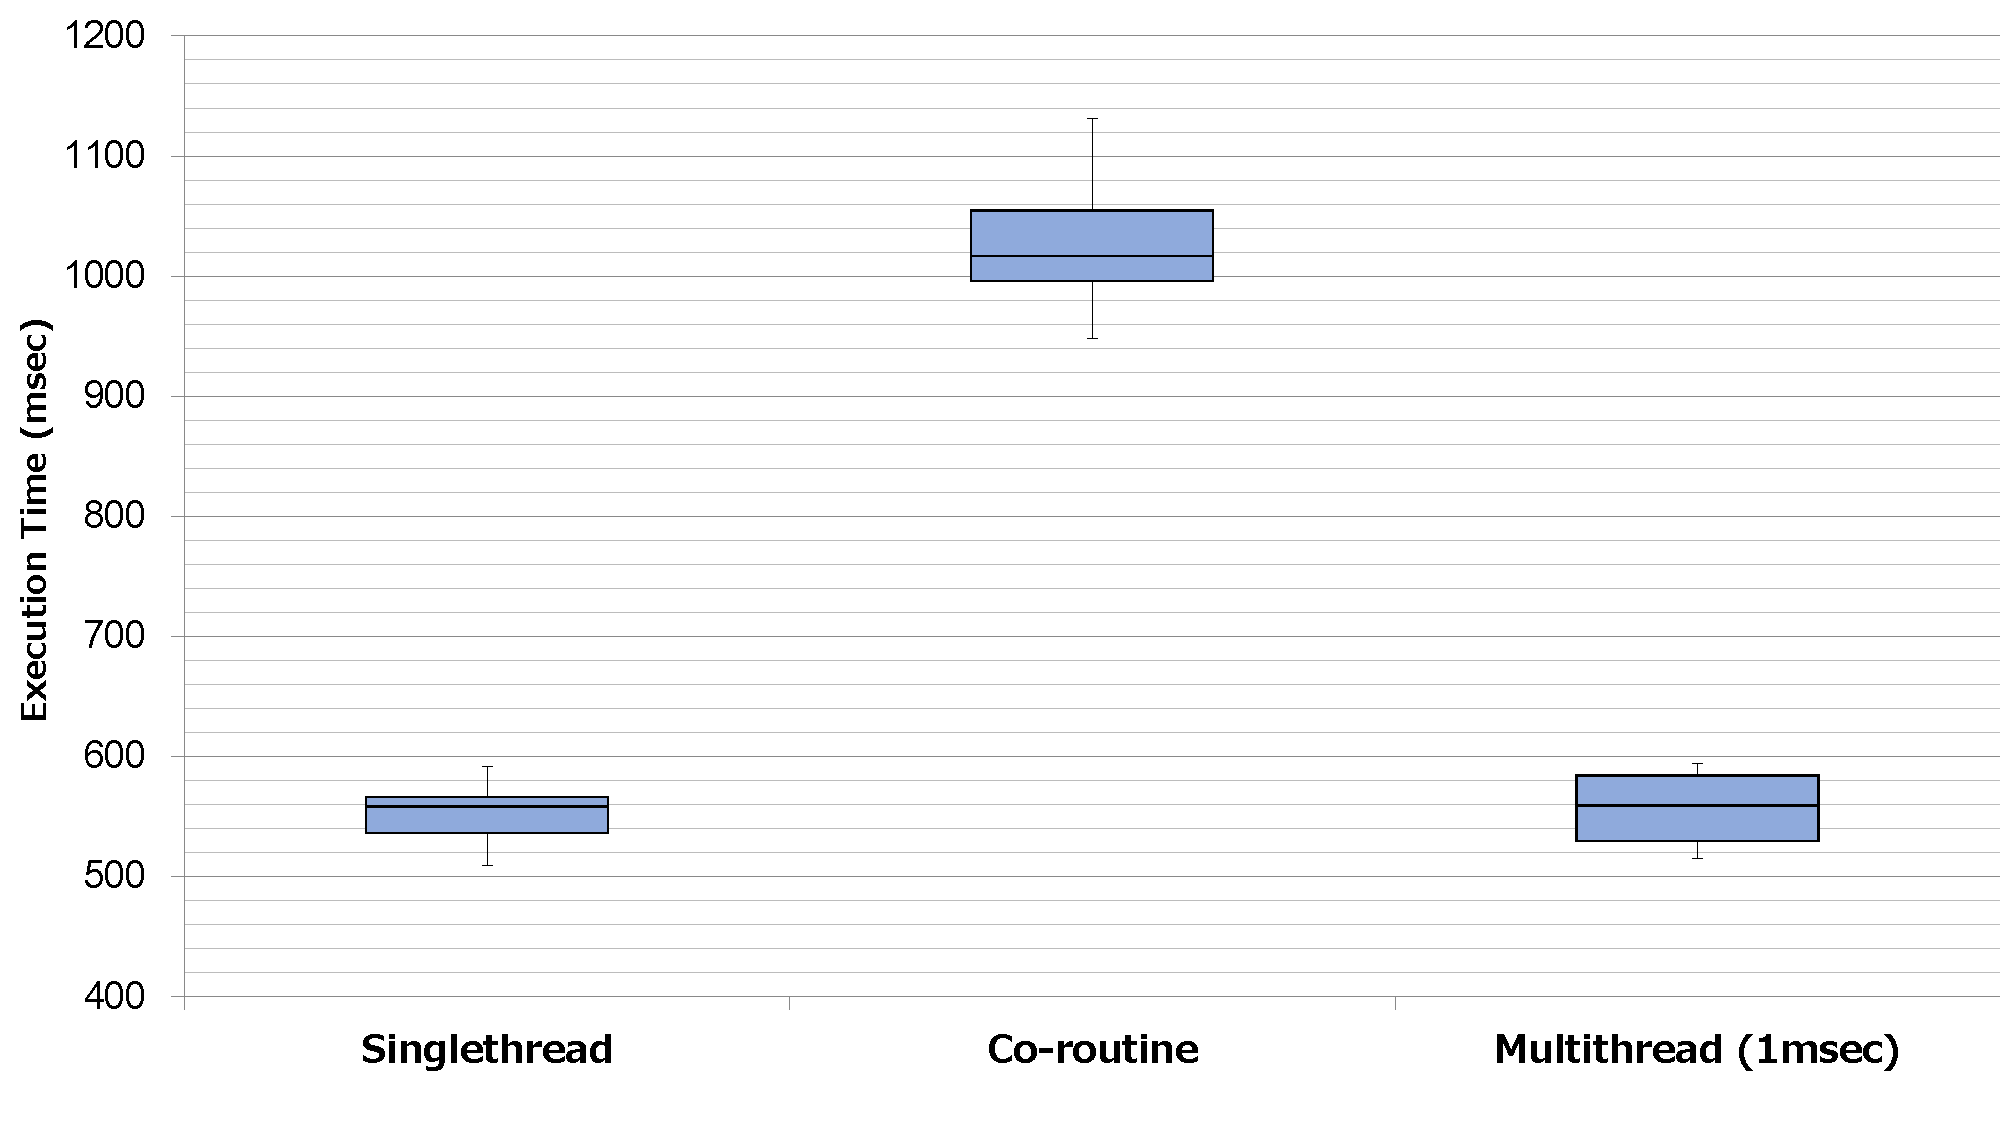
\includegraphics[width=8cm,clip]{figure/comparison_s_c_m.pdf}
    \caption{Comparison of the application execution time with singletask, co-routine, and multitask}
    \label{fig:comparison_s_c_m}
\end{figure}

Figure \ref{fig:comparison_msec} shows the execution time of multitasking with the cyclic handler.
A lower limit of the cyclic time is one msec due to the specification of TOPPERS/HRP2, the used RTOS.
More than 10 msec do not be evaluated in this paper because it is thought the larger cyclic time influences applications.
Each execution time of cyclic period is the same as the others.
That is because the overhead of switching tasks (about 3 $\mu$sec) is small in comparison with the execution time.
The smaller cyclic time is better in multitasking due to concurrent and/or parallel processing.

\begin{figure}[t]
    \centering
    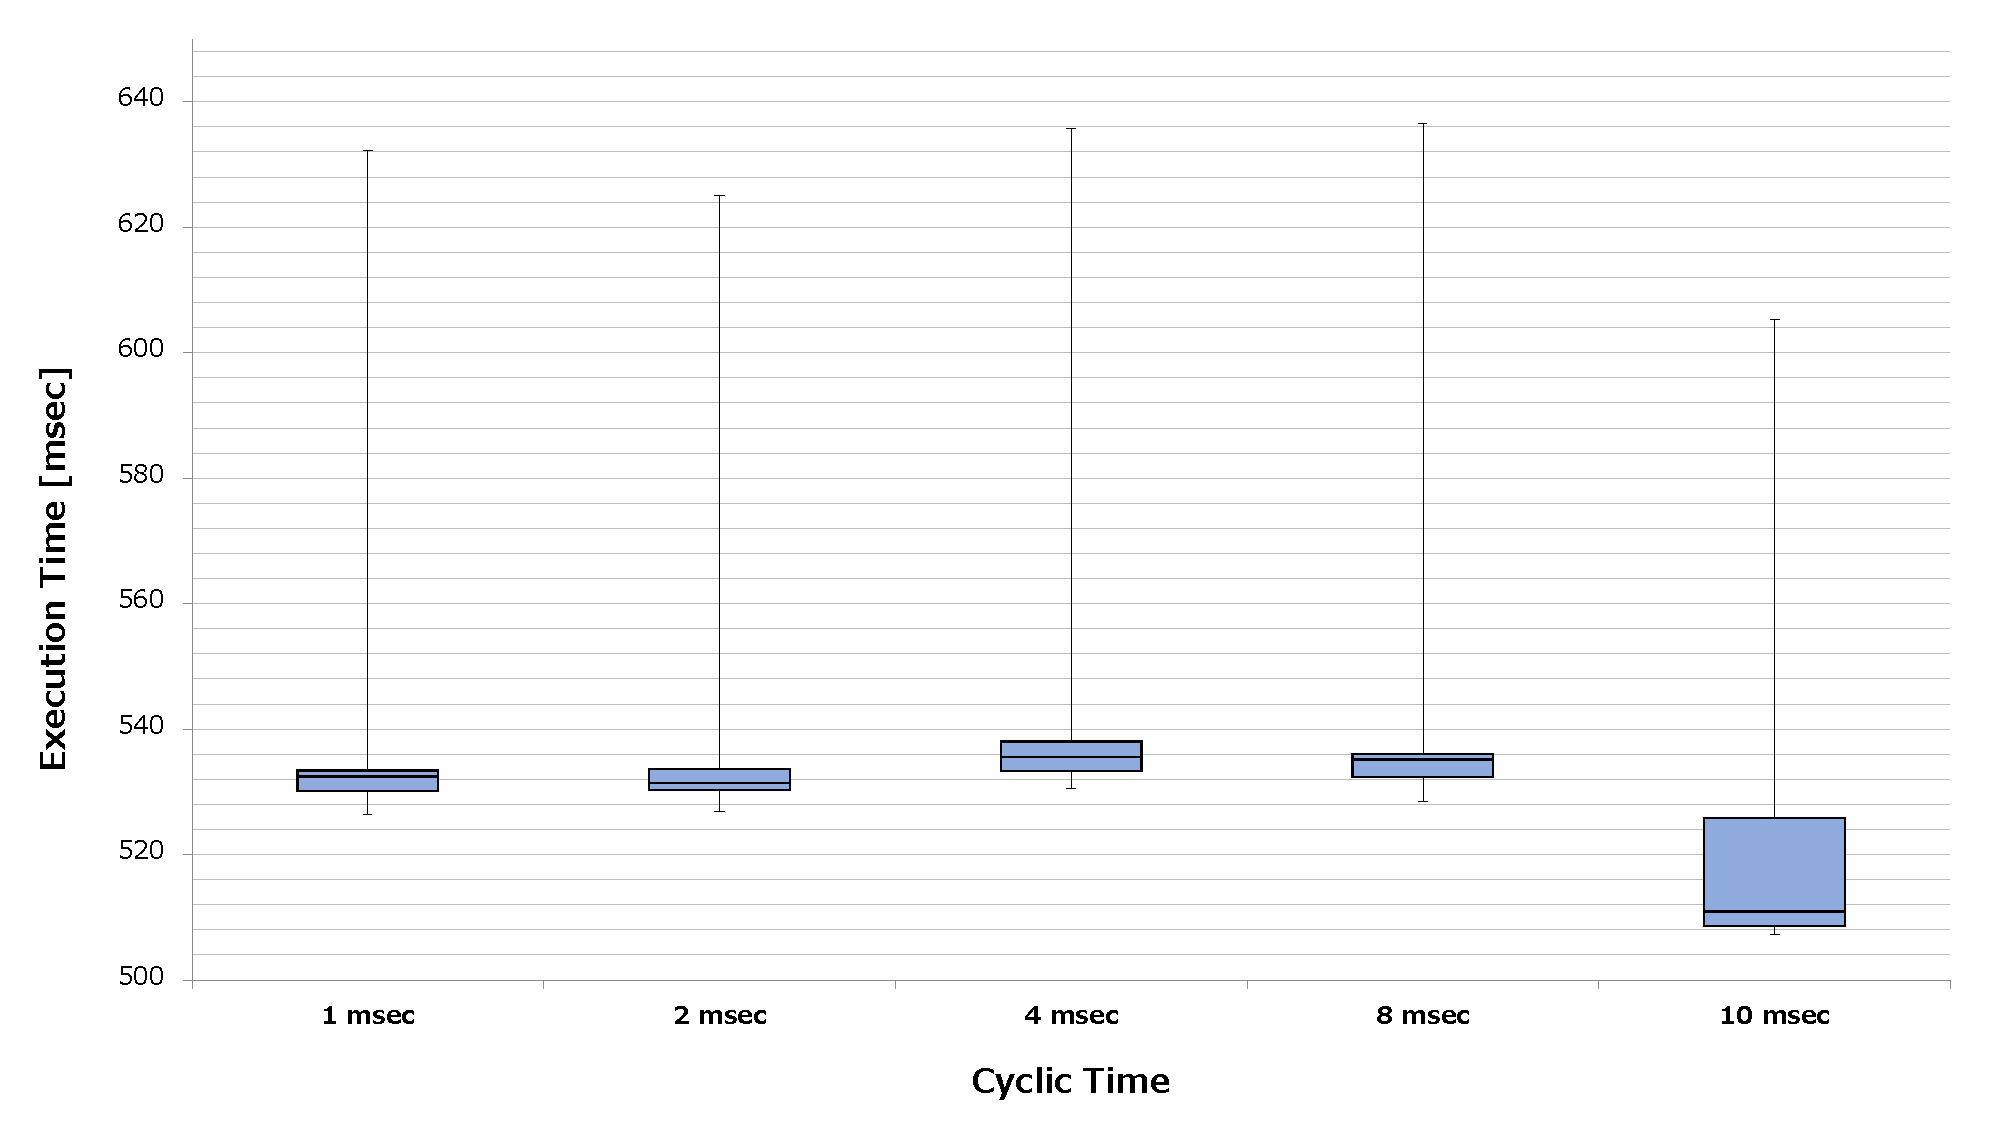
\includegraphics[width=8cm,clip]{figure/comparison_msec.pdf}
    \caption{Comparison of the overhead for each cyclic period of calling rotateReadyQueue}
    \label{fig:comparison_msec}
\end{figure}
 
\section{Related Work}
\label{sec:Related work}

\begin{table*}[t]
    \centering
    \caption{Comparion of the proposed and previous work}
    \begin{tabular}{c||c|ccc}
        & Bluetooth Loader & \shortstack{Preemptive-multitask\\(multi-VM)} & \shortstack{Nonpreemptive-multitask\\(co-routine)} & GIL \\ \hline
        Lua \cite{url:Lua}, \cite{par:Lua} &            & -          & \checkmark &            \\
        Owl system \cite{par:owl}                         &            & -          & -          & \checkmark \\
        mruby \cite{par:mruby}, \cite{url:mruby}                             &            &            & \checkmark &            \\
        mruby on TECS \cite{par:mrubyonTECS}                     &            & \checkmark & \checkmark &            \\
        Proposed framework& \checkmark & \checkmark & \checkmark &            \\
    \end{tabular}
    \label{tab:comparion}
\end{table*}
The open-source run-time systems for scripting languages have been proposed such as follow:
Lua \cite{url:Lua}, \cite{par:Lua}, the Owl system \cite{par:owl}, mruby \cite{par:mruby}, \cite{url:mruby}, and mruby on TECS \cite{par:mrubyonTECS}.

Lua is one of the most popular script languages for embedded systems.
Lua supports co-routine, referred to collaborative multitasking.
A co-routine in Lua is used as an independently executed thread.
A co-routine can just suspend and resume multiple routines.
Thus, a Lua co-routine is not like multitasks in multitask systems.

The Owl system is an embedded Python run-time system.
The Owl is a complete system for ARM Cortex-M3 microcontrollers.
The Owl toolchain produces relocatable memory images, that are directly runnable on the microcontroller, from Python code objects.
The interpreter of the Owl system is the same as that of python-on-a-chip \cite{url:python-on-a-chip}.
python-on-a-chip supports multitask managed by GIL (Global Interpreter Lock).
GIL locks a CPU in order to prevent the non-thread-safe code from sharing the other threads.
GIL leads the limitation of the concurrency on multitasking.

mruby, the lightweight implementation of the Ruby language, has been proposed for embedded systems.
mruby programs can run on a RiteVM, which is the VM for mruby and reads the mruby bytecode.
mruby has supported co-routine, but not supported multitasking for RTOSs.

mruby on TECS is a component-based framework for running mruby programs.
The programs on mruby on TECS can execute about 100 times faster than the mruby programs.
Software can be also developed with component base by mruby on TECS.
Although multitasking has been supported in the current mruby on TECS, developers need to be familiar with functions of an RTOS to use multitasking.
The co-routine is supported as same as mruby.

Table \ref{tab:comparion} shows a comparison between the proposed framework and previous work.
 
\section{Conclusion}
\label{sec:Conclusion}
This paper has presented the mruby bytecode loader using Bluetooth in multi-VM on mruby on TECS.
The proposed framework provides developers the efficient development without disconnecting an SD card and restarting an OS.
Furthermore, the proposed multitasking can be use more easily than the current mruby on TECS.
In the evaluation, experimental results of the mruby bytecode loader and proposed multitasking show their advantages.
mruby bytecode loader using Bluetooth can improve the work efficiency.
The proposed multitasking is compared with singletasking and co-routine.
This experimental result shows the effectiveness of the proposed framework because of the low overhead.

The proposed framework is developed in component-base by TECS.
The facilities such as the loader, the cyclic handler, and the eventflag are implemented as components.
Developers can easily add or remove the facilities as necessary.

In the future, the mruby bytecode loader using Bluetooth will be supported to handle multiple bytecodes and run the application in muliti-VM.
Moreover, the .cdl files for RiteVM and mruby-TECS bridge are generated automatically using a plugin, and developers can send a bytecode with ZMODEM protocol on the command line.
%%%%%%%%%%%%%
% Reference %
%%%%%%%%%%%%%
\bibliography{ref}

\end{document}
